\documentclass[runningheads]{llncs}





\usepackage{color}

\usepackage{graphicx}
\usepackage{tikz}
\usepackage{calc}

\usepackage{amsmath, amssymb}
\DeclareMathOperator*{\argmin}{arg\,min}

\usepackage{graphbox}
\usepackage{wasysym}

\usetikzlibrary{automata}




\title{On the power of oritatami cotranscriptional folding with unary bead sequence\thanks{This work is supported in part by KAKENHI Grant-in-Aid for Challenging Research (Exploratory) No.~18K19779 granted to S.~Z.~F. and S.~S. and JST Program to Disseminate Tenure Tracking System No.~6F36 granted to S.~S.}
}
\author{
Szil\'{a}rd Zsolt Fazekas\inst{1} \and
Shinnosuke Seki\inst{2}\thanks{Corresponding author}}
\institute{
Akita University, 
Graduate School of Engineering Science, 
1-1 Tegate Gakuen-machi, Akita, 0108502, Japan \\
\email{szilard.fazekas@ie.akita-u.ac.jp}
\and
The University of Electro-Communications, 
Graduate School of Informatics and Engineering, 
1-5-1 Chofugaoka, Chofu, Tokyo, 1828585, Japan \\
\email{s.seki@uec.ac.jp}
}

\begin{document}

\maketitle

\begin{abstract}
We investigate simple oritatami systems in an attempt to establish lower bounds on the size and complexity of computationally universal systems. 
In particular, we look at oritatami systems, where the folding sequence consists of a number of beads of the same type and show that under reasonable assumptions, these systems are not universal.
\end{abstract}

%------------------------------------------------------
	\section{Introduction}
%------------------------------------------------------

Transcription is the first essential step of gene expression, when a DNA template sequence is copied into a complementary single stranded RNA sequence by a `copy machine' called RNA polymerase. 
The RNA strand is synthesized letter by letter according to the complimentarity relation ${\tt A} \rightarrow {\tt U}$, ${\tt G} \rightarrow {\tt C}$, ${\tt C} \rightarrow {\tt G}$, and ${\tt T} \rightarrow {\tt A}$ and folds up during a process called co-transcriptional folding.

In a recent breakthrough in molecular engineering by Geary, Rothemund and Andersen~\cite{GearyRothemundAndersen2014} the co-transcriptional folding of RNA is controlled by careful design of the DNA template. As demonstrated in laboratory, this method, called RNA Origami, makes it possible to build rectangles out of RNA strands. 
Geary et al.~\cite{GeMeScSe2016} proposed a mathematical model for this process, called oritatami system.
It has been just shown in \cite{GeMeScSe2018} that the model is efficiently Turing universal by simulating cyclic tag systems introduced by Cook~\cite{Cook2004}. 
The simulation involves a very large and complex oritatami system. 
One future direction of research is to find smaller universal oritatami system.

Closely related is the question of where not to look for universal systems, i.e., what are the limitations of simple oritatami system. 
In search for simple oritatami systems, there are a number of restrictions one can pose on them:
\begin{itemize}
\item bounds on the delay, the number of bead types or the arity;
\item bounds on the size of the primary structure or of the attraction rule set;
\item structural conditions on the primary structure or the attraction rule set.
\end{itemize}

%Rogers and Seki~\cite{SimpleSim} showed that certain OS with small delays are not universal.

%Han, Kim, Rogers and Seki\cite{SelfRemove} proved that it is possible to avoid self-attraction rules without changing the behavior of OS.

In this paper we start a new line of study which concerns the alphabet size for the primary structure, i.e., the number of bead types.

\begin{figure}[tb]
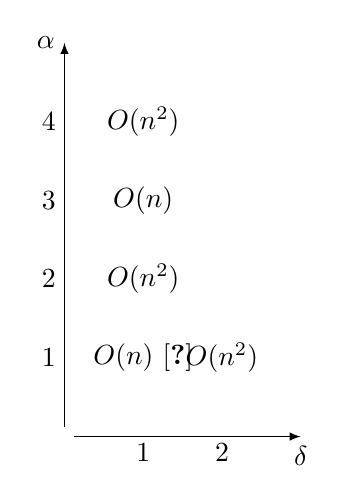
\begin{tikzpicture}

\node (origin) at (0, 0) {};

\draw[-latex] (origin) -- ++(0:3) node[below] {$\delta$}; 
\node at (1, -0.2) {1};
\node at (2, -0.2) {2};
\draw[-latex] (origin) -- ++(90:5) node[left] {$\alpha$}; 
\node at (-0.2, 1) {1};
\node at (-0.2, 2) {2};
\node at (-0.2, 3) {3};
\node at (-0.2, 4) {4};

%Results
\node at (1, 4) {$O(n^2)$};
\node at (1, 3) {$O(n)$};
\node at (1, 2) {$O(n^2)$};
\node at (1, 1) {$O(n)$ \cite{DemaineDNA24}};

\node at (2, 1) {$O(n^2)$};

\end{tikzpicture}
\caption{Summary of the results.}
\label{fig:summary}
\end{figure}

%------------------------------------------------------
	\section{Preliminaries}
%------------------------------------------------------
Let $\Sigma$ be a set of types of abstract molecules, or \textit{beads}. 
A bead of type $a \in \Sigma$ is called an $a$-bead. 
By $\Sigma^*$ and $\Sigma^\omega$, we denote the set of finite sequences of beads and that of one-way infinite sequences of beads, respectively. 
The empty sequence is denoted by $\lambda$. 
Let $w = b_1 b_2 \cdots b_n \in \Sigma^*$ be a sequence of length $n$ for some integer $n$ and bead types $b_1, \ldots, b_n \in \Sigma$. 
The \textit{length} of $w$ is denoted by $|w|$, that is, $|w| = n$. 
For two indices $i, j$ with $1 \le i \le j \le n$, we let $w[i..j]$ refer to the subsequence $b_i b_{i+1} \cdots b_{j-1}b_j$; if $i = j$, then $w[i..i]$ is simplified as $w[i]$. 
For $k \ge 1$, $w[1..k]$ is called a \textit{prefix} of $w$. 

Oritatami systems fold their transcript, which is a sequence of beads, over the triangular grid graph $\mathbb{T} = (V, E)$ cotranscriptionally. 
We designate one point in $V$ as the origin $O$ of $\mathbb{T}$. 
For a point $p \in V$, let $N_p^d$ denote the set of points which lie in the regular hexagon of radius $d$ centered at the point $p$. 
A directed path $P = p_1 p_2 \cdots p_n$ in $\mathbb{T}$ is a sequence of \textit{pairwise-distinct} points $p_1, p_2, \ldots, p_n \in V$ such that $\{p_i, p_{i+1}\} \in E$ for all $1 \le i < n$. 
Its $i$-th point is referred to as $P[i]$. 
Now we are ready to abstract RNA single-stranded structures in the name of conformation. 
A \textit{conformation} $C$ (over $\Sigma$) is a triple $(P, w, H)$ of a directed path $P$ in $\mathbb{T}$, $w \in \Sigma^*$ of the same length as $P$, and a set of h-interactions $H \subseteq \bigl\{\{i, j\} \bigm| 1 \le i, i+2 \le j, \{P[i], P[j]\} \in E \bigr\}$. 
This is to be interpreted as the sequence $w$ being folded along the path $P$ in such a manner that its $i$-th bead $w[i]$ is placed at the $i$-th point $P[i]$ and the $i$-th and $j$-th beads are bound (by a hydrogen-bond-based interaction) if and only if $\{i, j\} \in H$. 
The condition $i+2 \le j$ represents the topological restriction that two consecutive beads along the path cannot be bound. 
A \textit{rule set} $R \subseteq \Sigma \times \Sigma$ is a symmetric relation over $\Sigma$, that is, for all bead types $a, b \in \Sigma$, $(a, b) \in R$ implies $(b, a) \in R$. 
A bond $\{i, j\} \in H$ is \textit{valid with respect to $R$}, or simply $R$-valid, if $(w[i], w[j]) \in R$. 
This conformation $C$ is \textit{$R$-valid} if all of its bonds are $R$-valid. 
For an integer $\alpha \ge 1$, $C$ is \textit{of arity $\alpha$} if it contains a bead that forms $\alpha$ bonds but none of its bead forms more. 
By $\mathcal{C}_{\le \alpha}(\Sigma)$, we denote the set of all conformations over $\Sigma$ whose arity is at most $\alpha$; its argument $\Sigma$ is omitted whenever $\Sigma$ is clear from the context. 

The oritatami system grows conformations by an operation called elongation. 
Given a rule set $R$ and an $R$-valid conformation $C_1 = (P, w, H)$, we say that another conformation $C_2$ is an elongation of $C_1$ by a bead $b \in \Sigma$, written as $C_1 \xrightarrow{R}_b C_2$, if $C_2 = (P p, wb, H \cup H')$ for some point $p \in V$ not along the path $P$ and set $H' \subseteq \bigl\{ \{i, |w|+1\} \bigm| 1 \le i < |w|, \{P[i], p\} \in E, (w[i], b) \in R \bigr\}$ of bonds formed by the $b$-bead; this set $H'$ can be empty. 
Note that $C_2$ is also $R$-valid. 
This operation is recursively extended to the elongation by a finite sequence of beads as: for any conformation $C$, $C \xrightarrow{R}_\lambda^* C$; and for a finite sequence of beads $w \in \Sigma^*$ and a bead $b \in \Sigma$, a conformation $C_1$ is elongated to a conformation $C_2$ by $wb$, written as $C_1 \xrightarrow{R}_{wb}^* C_2$, if there is a conformation $C'$ that satisfies $C_1 \xrightarrow{R}_w^* C'$ and $C' \xrightarrow{R}_b C_2$. 

An \textit{oritatami system} (OS) $\Xi = (\Sigma, R, \delta, \alpha, \sigma, w)$ is composed of
\begin{itemize}
\item a set $\Sigma$ of bead types, 
\item a rule set $R \subseteq \Sigma \times \Sigma$, 
\item a positive integer $\delta$ called the \textit{delay}, 
\item a positive integer $\alpha$ called the \textit{arity}, 
\item an initial $R$-valid conformation $\sigma \in C_{\le \alpha}(\Sigma)$ called the \textit{seed}, upon which 
\item its (possibly infinite) \textit{transcript} $w \in \Sigma^* \cup \Sigma^\omega$ is to be folded by stabilizing beads of $w$ one at a time so as to minimize energy collaboratively with the succeeding $\delta{-}1$ nascent beads. 
\end{itemize}
The energy of a conformation $C = (P, w, H)$, denoted by $\Delta G(C)$, is defined to be ${-}|H|$; the more bonds a conformation has, the more stable it gets. 
The set $\mathcal{F}(\Xi)$ of conformations \textit{foldable} by the system $\Xi$ is recursively defined as: the seed $\sigma$ is in $\mathcal{F}(\Xi)$; and provided that an elongation $C_i$ of $\sigma$ by the prefix $w[1..i]$ be foldable (i.e., $C_0 = \sigma$), its further elongation $C_{i+1}$ by the next bead $w[i+1]$ is foldable if 
\begin{equation}\label{eq:OS_CF}
C_{i+1} \in \argmin_{
\substack{
C \in \mathcal{C}_{\le \alpha} s.t. \\
C_i \xrightarrow{R}_{w[i+1]}C \\
}
}
\min \Bigl\{ \Delta G(C') \Bigm|
C \xrightarrow{R}^*_{w[i+2...i+k]}C', k\le \delta, C' \in \mathcal{C}_{\le \alpha}
\Bigr\}.
\end{equation}
%
Then we say that the bead $w[i+1]$ and the bonds it forms are \textit{stabilized} according to $C_{i+1}$. 
Note that an arity-$\alpha$ oritatami system cannot fold any conformation of arity larger than $\alpha$. 
A conformation foldable by $\Xi$ is \textit{terminal} if none of its elongations is foldable by $\Xi$. 
The oritatami system $\Xi$ is \textit{deterministic} if for all $i \ge 0$, there exists at most one $C_{i+1}$ that satisfies \eqref{eq:OS_CF}. 
A deterministic oritatami system folds into a unique terminal conformation. 
An oritatami system with the empty rule set just folds into an arbitrary elongation of its seed nondeterministically. 
Thus, the rule set is always assumed to be non-empty. 

In the second half of this paper, we consider the unary oritatami system. 
An oritatami system is \textit{unary} if its bead type set $\Sigma$ is of size 1. 
Its sole bead type is denoted by $a$, that is, $\Sigma = \{a\}$. 
Its only possible rule is $(a, a)$ so that the non-empty rule set assumption implies that its rule set is $R = \{(a, a)\}$. 
Its transcript is a sequence of $a$-beads. 
That is to say, the behavior of a unary oritatami system is fully determined by the delay, arity, and seed. 





\begin{proposition}\label{prop:check_validity}
	For any rule set $R$, arity $\alpha$ and conformation $C = (P,w,H)$ it is possible to check whether $C$ is $R$-valid and whether $C\in \mathcal{C}_{\leq \alpha}$ in time $\mathcal{O}(|H|\cdot|w|\cdot|R|)$.
\end{proposition}
\begin{proof}
	To check whether $C$ is $R$-valid:
	\begin{enumerate}
		\item FOR each $(i,j)\in H$:
		\item \hspace{1cm} IF $(w[i],w[j])\notin R$ THEN answer NO and HALT
		\item answer YES and HALT
	\end{enumerate}	
	Checking the condition in 2. can be done in $\mathcal{O}(|w|\cdot|R|)$ time for any reasonable representation of $w$ and $R$, hence the whole process takes $\mathcal{O}(|H|\cdot |w|\cdot|R|)$ time.	
	To check the arity constraint $C\in \mathcal{C}_{\leq \alpha}$: 
	\begin{enumerate}
		\item FOR each $i\in \{1,\dots,|w|\}$:
		\item \hspace{1cm} IF $\mathrm{degree}(i)=|\{j | (i,j)\in H \}|>\alpha$ THEN answer NO and HALT
		\item answer YES and HALT
	\end{enumerate}	
	Checking the condition in 2. can be done in $\mathcal{O}(|H|)$ time for any reasonable representation of $H$, hence the whole process takes $\mathcal{O}(|w|\cdot|H|)$ time.
\end{proof}
\begin{theorem}\label{thm:OS_to_2dTM}
	There is an algorithm that simulates any oritatami system $\Xi = (\Sigma, R, \delta, \alpha, \sigma, w)$ in time $2^{\mathcal{O}(\delta)}\cdot |R|\cdot|w|$. 
\end{theorem}
\begin{proof}
	Take any step in the computation, up to which some $i \ge 0$ first beads of $w$ have been stabilized, with the last bead at a point $p$. 
	The number of all possible elongations of the current conformation by the next $\delta$-beads is $(6 \times 5^{\delta-1}) \times ((2^4)^{\delta-1} \times 2^5) \in 2^{O(\delta)}$. 
	By Proposition~\ref{prop:check_validity}, we can check for each of these elongations whether its arity is at most $\alpha$ or not and whether it is $R$-valid or not in time $\mathcal{O}((2^4)^{\delta-1}\cdot2^5\cdot \delta\cdot|R|)=2^{\mathcal{O}(\delta)}\cdot|R|$.  Therefore, the total running time is $2^{\mathcal{O}(\delta)}\cdot |R|\cdot|w|$.
\end{proof}

\begin{corollary}
	For fixed $\delta$ and $\alpha$, the class of problems solvable by oritatami systems $(\Sigma, R, \delta, \alpha, \sigma, w)$ is included in $\mathrm{DTIME}(n^3)$.
\end{corollary}
\begin{proof}
	The claim follows from Theorem~\ref{thm:OS_to_2dTM} and the fact that $|R|$ is implicitly bounded by $|w|^2$.
\end{proof}

%\begin{corollary}\label{polytranscript}
%	Let $k$ be a non-negative number. Let $\Sigma$, $H$, $\delta$, $\alpha$ be fixed and the transcript length bounded polynomially by the seed length, i.e., $|w|\in O(|\sigma|^k)$. Then, the language of seeds $\sigma$ accepted by an OS $(\Sigma, R, \delta, \alpha, \sigma, w)$ is in $\mathrm{DTIME}(|\sigma|^{2k})$.
%\end{corollary}

%If the transcript length is polynomially bounded by the seed length, than the accepted language is in $\mathrm{P}$. 

Because of the time hierarchy theorems, we know that $\mathrm{P}\subsetneq \mathrm{EXP}$, so we can conclude that OS which cannot deterministically fold transcripts of length exponential in the length of the seed are not computationally universal.

%-------------------------------------------------------
	\section{Problem description}
%-------------------------------------------------------

In \cite{DHOPRSST2018}, Demaine et al. proved that at delay 1 and arity 1, an oritatami system can fold upon the seed of size $n$ only the first $9n$ beads of a transcript deterministically. 
We consider this finiteness problem for unary oritatami systems under various settings of the values of delay and arity, which is formalized as follows. 

\begin{problem}\label{prob:det_unary_length}
Give an upper bound on the length of a transcript of a delay-$\delta$, arity-$\alpha$ deterministic unary oritatami system whose seed is of length $n$ by a function in $\delta$, $\alpha$, and $n$. 
\end{problem}



Results on this problem are summarized in Fig.~\ref{fig:summary}. 


\section{Case of arity $1$}




\subsection{$\alpha = 1$, arbitrary alphabets}
First we present a lower bound construction for arity $\alpha=1$ systems. At $\alpha=1$, allowing delay $\delta=2$ increases the power of OS compared with $\delta=1$, if at least four bead types are allowed. We demonstrate this with an infinite family of OS, which fold deterministically a transcript of length $\frac{(n-1)^2}{4}$ starting from a given seed of length $n$.

Consider the following $\delta=2$, $\alpha=1$ system with bead types $\{0,1,2,3,4\}$ and attraction rules $\{(1,1),(2,2), (3,3),(4,4)\}$. Let the seed $\sigma$ be a conformation of a $4k+1$ long bead sequence of the form $(1020)^k0$, such that bead $\sigma[i]$ of the seed is stabilized at point $(i,0)$, for all $1\leq i\leq 4k-1$. Bead $4k$ is at $(4k-1,-1)$ and bead $4k+1$ is at $(4k,0)$.

\noindent The transcript is
\begin{center}
	
	%\scriptsize
	\begin{tabular}{llll}
		& $k$ odd &  & $k$ even\\
		$w=$\hspace{1cm} & $(2413)^{k-1}241$ & \hspace{1cm} &  $(2413)^{k-1}241$\\
		     & $(4231)^{k-1}4$   & &  $(4231)^{k-1}4$  \\
		     & $(1324)^{k-2}132$ & &  $(1324)^{k-2}132$\\
		     & $(3142)^{k-2}3$   & &  $(3142)^{k-2}3$ \vspace{5pt}\\
		     
		     & $(2413)^{k-3}241$ & &  $(2413)^{k-3}241$\\
		     & $(4231)^{k-3}4$   & &  $(4231)^{k-3}4$  \\
		     & $(1324)^{k-4}132$ & &  $(1324)^{k-4}132$\\
		     & $(3142)^{k-4}3$   & &  $(3142)^{k-4}3$\\
			 & \vdots			 & &  \vdots\\
			 & $(2413)^{2} 241$	 & &  $(2413)^{1} 241$\\
			 & $(4231)^2 4$		 & &  $(4231)^1 4$\\
			 & $(1324)^1 132$	 & &  $(1324)^0 132$\\
			 & $(3142)^1 3$		 & &  $(3142)^0 3$\\
			 & $(2413)^0 241$	 & & \\
			 & $(4231)^0 4$  	 & 
	\end{tabular}
	
\end{center}
The transcript above is written in rows which correspond to beads in the conformation stabilized along the same row on the grid. To simplify the argument we will use \textit{row} both for the transcript above and for the conformation it stabilizes in. In line with this, row $\ell\in \{1,\dots, 2k\}$ is as follows:  
\begin{center}
	\begin{tabular}{llll}
							& row $\ell$ & 			& $\ell\mod 4$ \\
			& $(2413)^{k-\lfloor (\ell+1)/2\rfloor}241$ & \hspace{1cm} &  $\ell\equiv 1\mod 4$\\
							& $(4231)^{k-\lfloor (\ell+1)/2\rfloor}4$   & &  $\ell\equiv 2 \mod 4$ \\
							& $(1324)^{k-\lfloor (\ell+1)/2\rfloor}132$ & &  $\ell\equiv 3 \mod 4$\\
							& $(3142)^{k-\lfloor (\ell+1)/2\rfloor}3$   & &  $\ell\equiv 4 \mod 4$ 
	\end{tabular}
\end{center}
so $w=\mathrm{row}_1\cdots \mathrm{row}_{2k}$. Row $1$ is of length $4k-1$ and row $\ell+1$ is two beads shorter than row $\ell$, so the length of the whole transcript is $|w|=4k^2=\frac{(4k+1-1)^2}{4}=\frac{(|\sigma|-1)^2}{4}$. As an example, see Fig.~\ref{CI:big}, where $k=5$, so the length of the seed is $4k+1=21$ and the transcript is $4k^2 = 100$ beads long.

\begin{figure}
	\centering
	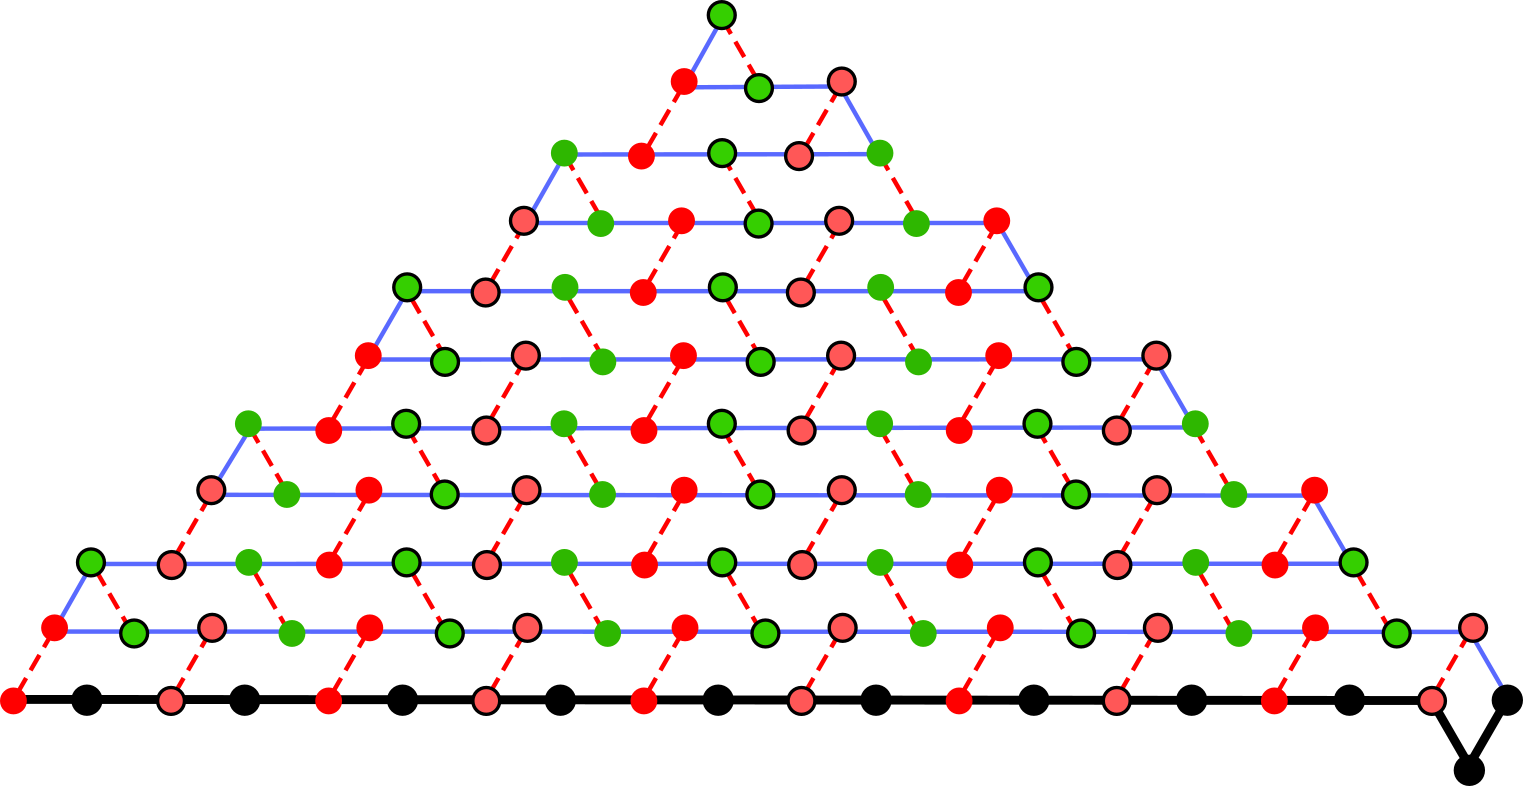
\includegraphics[width=0.9\linewidth]{./Fig/chichenBig}
	\caption{Quadratic length transcript folding deterministically into pyramid shape. Seed: thick black path. Transcript: thin blue path. Bonds: dashed red lines. Beads: '$0$' black, '$1$' red, '$2$' red with black contour, '$3$' green, '$4$' green with black contour.}
	\label{CI:big}
\end{figure}


Stabilizing the first bead of row $j$ goes as follows (see Fig.~\ref{CI:turn}):
%\begin{itemize}
%	\item $\bf j\equiv 1\mod 4$: the first two beads are $24$, and the preceding bead is stabilized at $(4k-\frac{j-1}{2}, j-1)$. The $2$ can only bind to the $2$ which occurred two beads before at $(4k-\frac{j+1}{2}, j-1)$, and $4$ cannot bind anywhere, so the $2$ is stabilized at $(4k-\frac{j-1}{2},j)$.
%\end{itemize}

\begin{center}
	\begin{tabular}{|c|c|c|c|c|@{}m{0pt}@{}}
		%\renewcommand{\arraystretch}{2}
	$j\mod 4$					& first bead 	& predecessor at		& first bead binds to		& first stabilizes at\\
						\hline
	$\equiv 1$	& 2		& $(4k-\frac{j-1}{2}, j-1)$		& $(4k-\frac{j+1}{2}, j-1)$	& $(4k-\frac{j+1}{2}, j)$& $\mathrm{ }$\newline $\mathrm{ }$\\
	\hline
	$\equiv 2$	& 4				& $(\frac{3j}{2}-1,j-1)$		& $(\frac{3j}{2},j-1)$		& $(\frac{3j}{2},j)$ & $\mathrm{ }$\newline $\mathrm{ }$\\
	\hline
	$\equiv 3$	& 1				& $(4k-\frac{j-1}{2}, j-1)$		& $(4k-\frac{j+1}{2}, j-1)$	& $(4k-\frac{j+1}{2}, j)$ & $\mathrm{ }$\newline $\mathrm{ }$ \\
	\hline
	$\equiv 4$	& 3				& $(\frac{3j}{2}-1,j-1)$		& $(\frac{3j}{2},j-1)$		& $(\frac{3j}{2},j)$ & $\mathrm{ }$\newline $\mathrm{ }$ \\
	\hline		
	\end{tabular}
\end{center}



%The first bead of the transcript is type $2$ and it has to be fixed next to $(4k,0)$. The second bead is type $4$, which cannot form a bond with anything in the conformation so far. The only possibility of forming a bond is if the $2$-bead is placed at $(4k,1)$ and it bonds with the $2$-bead of the seed at $(4k-1,0)$. The next to be stabilized is a $4$-bead, and since it cannot form any bond, the conformation with the highest number of bonds is when the one after, a $1$-bead, is at $(4k-2,1)$ bonding with $(4k-3,0)$, which stabilizes the preceding $4$-bead at $(4k-1,1)$ (see Fig.~\ref{CI:1-4}, (a)-(b)).



\begin{figure}
	\begin{minipage}{.35\textwidth}
		\centering
		\includegraphics[align=c,height=1in]{./Fig/CI_1}\\
		\bigskip
		
		(a) First transcript bead
	\end{minipage}%
	\begin{minipage}{.2\textwidth}
		\centering
		\includegraphics[align=c,height=0.7in]{./Fig/CI_2}\\
		\bigskip
		
		(b) Second bead
	\end{minipage}
	\begin{minipage}{.4\textwidth}
		\centering
		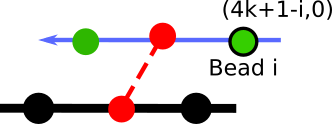
\includegraphics[align=c,height=0.5in]{./Fig/CI_3}
		\bigskip
		\vspace{0.1in}
		\includegraphics[align=c,height=0.5in]{./Fig/CI_4}
		\bigskip
		
		(c) Bead $i+1$, when bead $i$ is $B_{3,4}$ and $B_{1,2}$, respectively
	\end{minipage}
	\caption{Fixing transcript beads in odd rows}
	\label{CI:1-4}
\end{figure}


As for the other beads, in rows $j\equiv 1,3\mod 4$, beads of type $1$ and $3$ bind to a bead in row $j-1$. In rows $j\equiv 2,4\mod 4$ beads of type $2$ and $4$ can bind to a bead in row $j-1$.  This is true for row $1$, because beads of type $1$ and $3$ from row $1$ can only bind to every second bead of the seed, whereas beads of type $2$ and $4$ from row $1$ cannot bind to anything (Fig.~\ref{CI:1-4}, (c)). Once this dynamic holds for a row, it holds inductively for the next, as a bead that binds to another loses its only free hand at arity $1$.

Within one row of the transcript, no bead can bind to a preceding bead, because if there is a previous bead of the same type in that row, it is stabilized at a distance of four and the system has delay $2$.

By the arguments above, the beads in row $i$ of the transcript are stabilized along row $i$ on the grid, forming the pyramid-like conformation from Fig.~\ref{CI:big}.


\begin{figure}
	\centering
	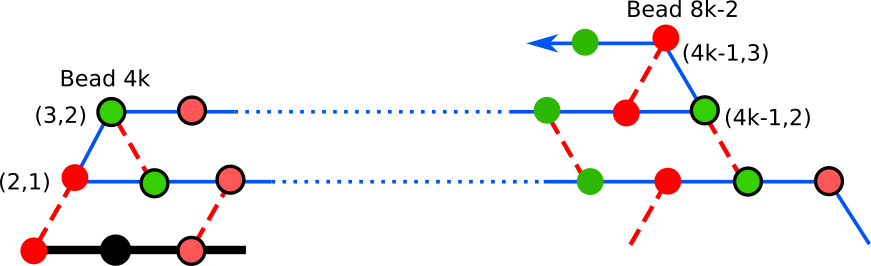
\includegraphics[width=0.7\linewidth]{./Fig/CI_turn}
	\caption{Beads $4k, 8k-2, \dots$ stabilize at turning points because the bead two positions before is the same type and has a free hand.}
	\label{CI:turn}
\end{figure}




\subsection{$\alpha = 1$, unary}

Let the point where the first transcript bead was fixed be $p$ and let $n=|\mathrm{seed}|+1$. We will argue about the situation when the first bead is stabilized outside $\hexagon_p^n$ (a hexagon of radius $n$). Let this be the $i$th bead of the transcript. Without loss of generality, we can translate the origin $(0,0)$ to the coordinates of bead $i-1$ (which is still in $\hexagon_p^n$), and we can assume that the bead outside the hexagon is fixed at $(1,1)$ (see Fig.~\ref{fig:hexagonOut}).
\begin{figure}
	\centering
	\includegraphics[width=0.3\linewidth]{./Fig/hexagonOut}
	\caption{$\hexagon_p^n$ and the position $(1,1)$ of the first bead fixed outside of it.}
	\label{fig:hexagonOut}
\end{figure}

In the elongation that places bead $i$ at $(1,1)$ there are two possibilities:
\begin{itemize}
	\item $i$ forms a bond with a bead at $(1,0)$.
	\item  $i$ does not bond to anything and $i+1$ is at $(2,1)$ bonding with a bead at $(2,0)$. If there is no bead at $(1,0)$, then placing $i$ at $(1,0)$ instead of $(1,1)$ results in the same number of bonds, leading to nondeterminism. Therefore, there has to be a bead at $(1,0)$ and it is inactive, otherwise it would bond to $i$. This is analogous to case 1. below.%as in Fig.~\ref{fig:hexagonOut1}.
	\begin{figure}
		\centering
		\includegraphics[width=0.2\linewidth]{./Fig/hexagonOut1}
		%\caption{}
		\label{fig:hexagonOut1}
	\end{figure}
	
\end{itemize}
 
%The only position with which $(1,1)$ can form a bond is $(1,0)$. This means that there is a bead at $(1,0)$, which bonds to bead $i$, otherwise there are other conformations in which beads $i$ and $i+1$ add one bond to the conformation, making the behavior nondeterministic.

The next bead, $i+1$, can be fixed at $(2,1)$ or at $(0,1)$ as all other possibilities result in nondeterministic behavior immediately, so we have two cases.

\begin{enumerate}
	\item bead $i+1$ is fixed at $(2,1)$ and can bond with a bead at $(2,0)$. Now consider bead $i+2$. For $i+1$ to be fixed at $(2,1)$, $i+2$ needs to form a bond somewhere, otherwise $i+2$ could go to $(2,1)$ forming the bond with the bead at $(2,0)$ and there would be two conformations with the maximal $1$ bond. The only possibility is that there is a bead at $(3,0)$ and $i+2$ can bond with it when placed at $(3,1)$. We can apply the same argument inductively: there is some $m\geq 0$ such that grid points $(\ell,0)$ are occupied by active beads, for all $\ell\in \{2,\dots,2+m\}$, and there is no bead at $(3+m,0)$. Such an $m$ exists, and it is not greater than $n$. Then, bead $i+\ell$ is fixed at $(\ell+1,1)$ and bonds with $(\ell+1,0)$. However, bead $i+2+m$ cannot be fixed anywhere, because $i+2+m$ and $i+3+m$ can only add one bond to the conformation, and that is possible either with $i+2+m \rightarrow (2+m,1)$, $i+3+m \rightarrow (3+m,1)$ or with $i+2+m \rightarrow (2+m,2)$, $i+3+m \rightarrow (2+m,1)$. 
	\begin{figure}
		\centering
		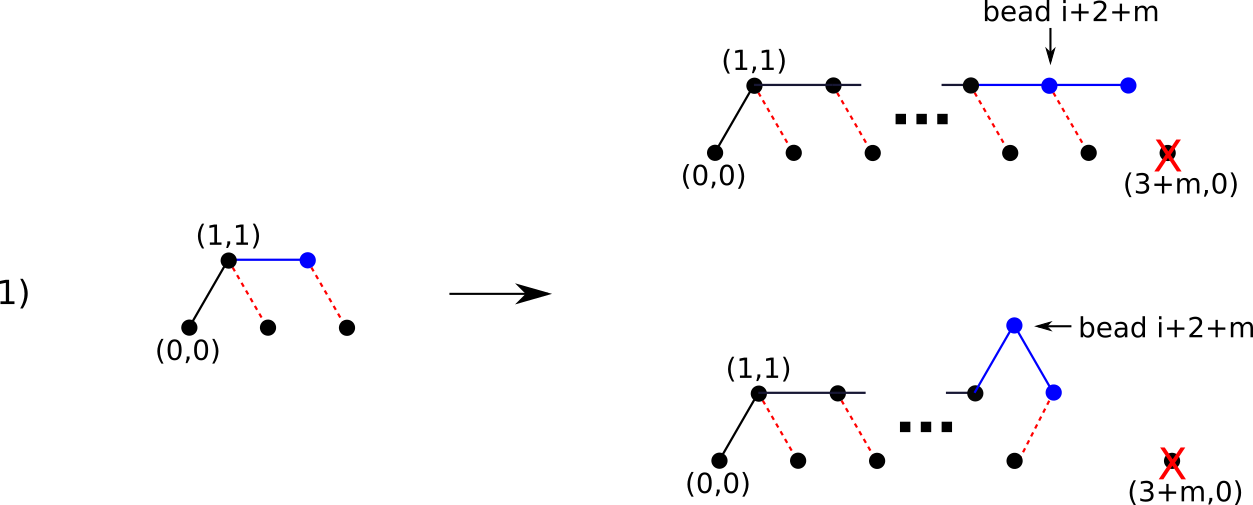
\includegraphics[width=0.6\linewidth]{./Fig/hexagonOut2}
		\caption{}
		\label{fig:hexagonout2}
	\end{figure}
	
	\item bead $i+1$ is fixed at $(0,1)$. This is only possible if
	\begin{enumerate}
		\item there is an inactive bead at $(-1,0)$ and an active one at $(-2,0)$. This case is symmetrical to (1).
		\item there is no bead at $(-1,0)$, bead $i+1$ can bond with bead $i-1$ at $(0,0)$ and the bead $i+2$ can be placed at $(-1,0)$ where it can bond with $(-2,0)$, $(-2,-1)$ or $(-1,-1)$. This leads to nondeterminism, because bead $i$ at $(-1,0)$ and bead $i+1$ at $(0,1)$ has two bonds, just as the original conformation.
		\item there is a bead at $(-1,0)$ and bead $i+1$ can bond with that or with bead $i-1$ at $(0,0)$. However, this means that placing bead $i$ at $(0,1)$ at bead $i+1$ at $(1,1)$ creates the same number of hydrogen bonds, thus resulting in bead $i$ not being placed deterministically.
		
	\end{enumerate}
\end{enumerate}




\begin{figure}
	\centering
	%\includegraphics[width=0.3\linewidth]{./hexagonOut1}
	%\hspace{10mm} %
	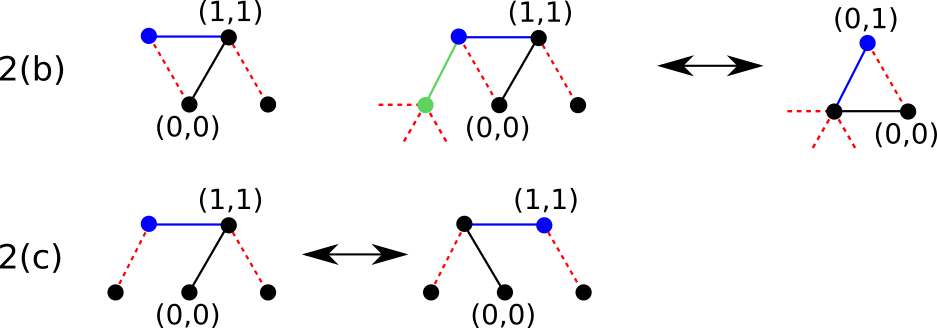
\includegraphics[width=0.6\linewidth]{./Fig/hexagonOut3}
	
	\caption{}
	\label{fig:hexagonOut2}
\end{figure}


\subsection{In the case of $\delta = 3$}

As before, the length of seed is $n$ and the seed will be inside $\hexagon_p^n$, the equilateral hexagon with a radius of $n$ and center $p$, the point where the first bead of the seed is fixed. We will begin our discussion by considering the moment when the first bead is fixed outside $\hexagon_p^n$. Let this bead be the $i$th one. 

\textbf{A.} First, let us assume that a fixed bead on a side of $\hexagon_p^n$ has a free hand, and bead $i$ binds to it. If the most stable conformation formed by beads $i, i+1, i+2$ has only two hydrogen bonds, it will be nondeterministic because there are at least two possibilities, see Fig.~\ref{fig:beadi}. Therefore, it needs to make three hydrogen bonds to deterministically stabilize $i$.\\

\begin{figure}
  \begin{center}
  \begin{tabular}{cc}
    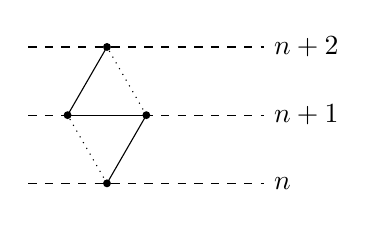
\begin{tikzpicture}
      \draw [dashed] (-1.0, 0.0) -- (2.0, 0.0);
      \fill (2.0, 0.0) node [right] {$n$};
      \draw [dashed] (-1.0, 0.866) -- (2.0, 0.866);
      \fill (2.0, 0.866) node [right] {$n+1$};
      \draw [dashed] (-1.0, 1.732) -- (2.0, 1.732);
      \fill (2.0, 1.732) node [right] {$n+2$};
      \fill (0,0) circle [radius = 0.05];
      \begin{scope}[shift = (0 : 0.0)]
        \foreach \theta in {60, 120}{
          \fill (0,0) [transform canvas = {shift = (\theta : 1.0)}] circle [radius = 0.05];
        }
        \draw (0 : 0.0) -- (60 : 1.0);
        \draw (60 : 1.0) -- (120 : 1.0);
        \draw [dotted] (0 : 0.0) -- (120 : 1.0);
      \end{scope}
      \begin{scope}[shift = (60 : 1.0)]
        \draw [dotted] (0 : 0.0) -- (120 : 1.0);
      \end{scope}
      \begin{scope}[shift = (120 : 1.0)]
        \foreach \theta in {60}{
        \fill (0,0) [transform canvas = {shift = (\theta : 1.0)}] circle [radius = 0.05];
        }
        \draw (0 : 0.0) -- (60 : 1.0);
      \end{scope}
    \end{tikzpicture}

    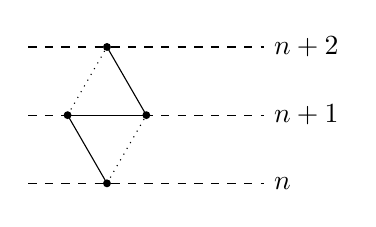
\begin{tikzpicture}
      \draw [dashed] (-1.0, 0.0) -- (2.0, 0.0);
      \fill (2.0, 0.0) node [right] {$n$};
      \draw [dashed] (-1.0, 0.866) -- (2.0, 0.866);
      \fill (2.0, 0.866) node [right] {$n+1$};
      \draw [dashed] (-1.0, 1.732) -- (2.0, 1.732);
      \fill (2.0, 1.732) node [right] {$n+2$};
      \fill (0,0) circle [radius = 0.05];
      \begin{scope}[shift = (0 : 0.0)]
        \foreach \theta in {60, 120}{
          \fill (0,0) [transform canvas = {shift = (\theta : 1.0)}] circle [radius = 0.05];
        }
        \draw [dotted] (0 : 0.0) -- (60 : 1.0);
        \draw (60 : 1.0) -- (120 : 1.0);
        \draw (0 : 0.0) -- (120 : 1.0);
      \end{scope}
      \begin{scope}[shift = (60 : 1.0)]
        \draw (0 : 0.0) -- (120 : 1.0);
      \end{scope}
      \begin{scope}[shift = (120 : 1.0)]
        \foreach \theta in {60}{
        \fill (0,0) [transform canvas = {shift = (\theta : 1.0)}] circle [radius = 0.05];
        }
        \draw [dotted](0 : 0.0) -- (60 : 1.0);
      \end{scope}
    \end{tikzpicture}
    \end{tabular}
    \caption{}
    \label{fig:beadi}
  \end{center}
\end{figure}

There are the two cases in which beads $i, i+1, i+2$ can have three bonds, see Fig.~\ref{fig:3bonds}. However, if it makes three bonds once, such as in Fig.~\ref{fig:3bonds}, it will need to make three bonds forever to be deterministic. Similarly to case 1. in the previous section, this becomes nondeterministic finally, as in Fig.~\ref{fig:hexcorner}, when it reaches a corner of $\hexagon_p^n$. Thus, the fixed bead on the side of an equilateral hexagon with a radius of $n$ has to make a hydrogen bond with a bead in an equilateral hexagon.

\begin{figure}
  \begin{center}
  \begin{tabular}{cc}
    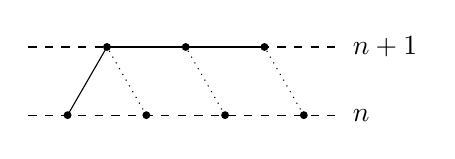
\begin{tikzpicture}
      \draw [dashed] (-0.5, 0.0) -- (3.5, 0.0);
      \fill (3.5, 0.0) node [right] {$n$};
      \draw [dashed] (-0.5, 0.866) -- (3.5, 0.866);
      \fill (3.5, 0.866) node [right] {$n+1$};
      \fill (0,0) circle [radius = 0.05];
      \begin{scope}[shift = (0 : 0.0)]
        \foreach \theta in {0, 60}{
          \fill (0,0) [transform canvas = {shift = (\theta : 1.0)}] circle [radius = 0.05];
        }
        \draw (0 : 0.0) -- (60 : 1.0);
      \end{scope}
      \begin{scope}[shift = (0 : 2.0)]
        \fill (0,0) circle [radius = 0.05];
        \foreach \theta in {0, 60, 120}{
          \fill (0,0) [transform canvas = {shift = (\theta : 1.0)}] circle [radius = 0.05];
        }
        \draw [dotted] (0 : 0.0) -- (120 : 1.0);
      \end{scope}
      \begin{scope}[shift = (60 : 1.0)]
          \draw (0 : 0.0) -- (0 : 2.0);
      \end{scope}
      \begin{scope}[shift = (0 : 1.0)]
          \draw [dotted] (0 : 0.0) -- (120 : 1.0);
      \end{scope}
      \begin{scope}[shift = (0 : 3.0)]
          \draw [dotted] (0 : 0.0) -- (120 : 1.0);
      \end{scope}
    \end{tikzpicture}

    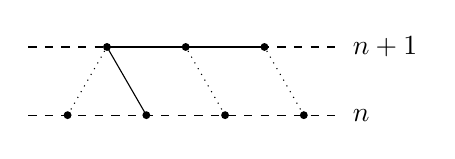
\begin{tikzpicture}
      \draw [dashed] (-1.5, 0.0) -- (2.5, 0.0);
      \fill (2.5, 0.0) node [right] {$n$};
      \draw [dashed] (-1.5, 0.866) -- (2.5, 0.866);
      \fill (2.5, 0.866) node [right] {$n+1$};
      \fill (0,0) circle [radius = 0.05];
      \begin{scope}[shift = (0 : 0.0)]
        \foreach \theta in {0, 60, 120, 180}{
          \fill (0,0) [transform canvas = {shift = (\theta : 1.0)}] circle [radius = 0.05];
        }
        \draw (0 : 0.0) -- (120 : 1.0);
      \end{scope}
      \begin{scope}[shift = (0 : 2.0)]
        \fill (0,0) circle [radius = 0.05];
        \foreach \theta in {120}{
          \fill (0,0) [transform canvas = {shift = (\theta : 1.0)}] circle [radius = 0.05];
        }
        \draw [dotted] (0 : 0.0) -- (120 : 1.0);
      \end{scope}
      \begin{scope}[shift = (120 : 1.0)]
          \draw (0 : 0.0) -- (0 : 2.0);
      \end{scope}
      \begin{scope}[shift = (0 : 1.0)]
          \draw [dotted] (0 : 0.0) -- (120 : 1.0);
      \end{scope}
      \begin{scope}[shift = (180 : 1.0)]
          \draw [dotted] (0 : 0.0) -- (60 : 1.0);
      \end{scope}
    \end{tikzpicture}
    \end{tabular}
    \caption{}
    \label{fig:3bonds}
  \end{center}
  	
\end{figure}

\begin{figure}
  \begin{center}
  \begin{tabular}{cc}
    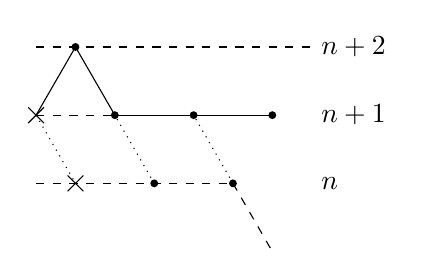
\begin{tikzpicture}
      \draw [dashed] (-0.5, 0.0) -- (2.0, 0.0);
      \fill (3.0, 0.0) node [right] {$n$};
      \draw [dashed] (-0.5, 0.866) -- (2.5, 0.866);
      \fill (3.0, 0.866) node [right] {$n+1$};
      \draw [dashed] (-0.5, 1.732) -- (3.0, 1.732);
      \fill (3.0, 1.732) node [right] {$n+2$};
      \fill (60 : 1.0) circle [radius = 0.05];
      \draw (-0.1,-0.1) -- (0.1,0.1);
      \draw (0.1,-0.1) -- (-0.1,0.1);
      \begin{scope}[shift = (120 : 1.0)]
        \draw (-0.1,-0.1) -- (0.1,0.1);
        \draw (0.1,-0.1) -- (-0.1,0.1);
      \end{scope}
      \begin{scope}[shift = (120 : 1.0)]
        \draw [dotted] (0 : 0.0) -- (300 : 1.0);
      \end{scope}
      \begin{scope}[shift = (60 : 1.0)]
        \draw (0.0, 0.0) -- (2.0, 0.0);
        \fill (2.0, 0.0) circle [radius = 0.05];
      \end{scope}
      \begin{scope}[shift = (0 : 2.0)]
        \draw [dashed] (0 : 0.0) -- (300 : 1.0);
      \end{scope}
      \begin{scope}[shift = (0 : 1.0)]
      \fill (0.0, 0.0) circle [radius = 0.05];
        \foreach \theta in {0, 60}{
          \fill (0,0) [transform canvas = {shift = (\theta : 1.0)}] circle [radius = 0.05];
        }
        \draw [dotted] (0 : 0.0) -- (120 : 1.0);
      \end{scope}
      \begin{scope}[shift = (0 : 2.0)]
        \draw [dotted] (0 : 0.0) -- (120 : 1.0);
      \end{scope}
      \begin{scope}[shift = (60 : 1.0)]
        \begin{scope}[shift = (120 : 1.0)]
          \fill (0.0, 0.0) circle [radius = 0.05];
          \draw (0 : 0.0) -- (240 : 1.0);
          \draw (0 : 0.0) -- (300 : 1.0);
        \end{scope}
      \end{scope}
    \end{tikzpicture}

    \begin{tikzpicture}
      \draw [dashed] (-0.5, 0.0) -- (2.0, 0.0);
      \fill (3.0, 0.0) node [right] {$n$};
      \draw [dashed] (-0.5, 0.866) -- (2.5, 0.866);
      \fill (3.0, 0.866) node [right] {$n+1$};
      \draw (-0.1,-0.1) -- (0.1,0.1);
      \draw (0.1,-0.1) -- (-0.1,0.1);
      \fill (60 : 1.0) circle [radius = 0.05];
      \begin{scope}[shift = (120 : 1.0)]
        \draw (-0.1,-0.1) -- (0.1,0.1);
        \draw (0.1,-0.1) -- (-0.1,0.1);
      \end{scope}
      \begin{scope}[shift = (120 : 1.0)]
        \draw [dotted] (0 : 0.0) -- (300 : 1.0);
        \draw (0.0, 0.0) -- (3.0, 0.0);
      \end{scope}
      \begin{scope}[shift = (0 : 2.0)]
        \draw [dashed] (0 : 0.0) -- (300 : 1.0);
        \fill (60 : 1.0) circle [radius = 0.05];
      \end{scope}
      \begin{scope}[shift = (0 : 1.0)]
        \fill (0.0, 0.0) circle [radius = 0.05];
        \foreach \theta in {0, 60}{
          \fill (0,0) [transform canvas = {shift = (\theta : 1.0)}] circle [radius = 0.05];
        }
        \draw [dotted] (0 : 0.0) -- (120 : 1.0);
      \end{scope}
      \begin{scope}[shift = (0 : 2.0)]
        \draw [dotted] (0 : 0.0) -- (120 : 1.0);
      \end{scope}
    \end{tikzpicture}
    \end{tabular}
    \caption{}
    \label{fig:hexcorner}
  \end{center}
\end{figure}

\textbf{B.} Next, assume that bead $i$ could not bind to anything and let us discuss the moment after bead $i$ is fixed outside $\hexagon_p^n$. Now bead $i$ has a free hand. If beads $i+1, i+2, i+3$ can form only two bonds, it will be nondeterministic because there are at least two possible such structures, as in Fig.~\ref{fig:afterzigzag}. Hence, they need to form three bonds to deterministically stabilize, such as in the right or left side of Fig.~\ref{fig:afterline}.\\

\begin{figure}
  \begin{center}
  \begin{tabular}{cc}
    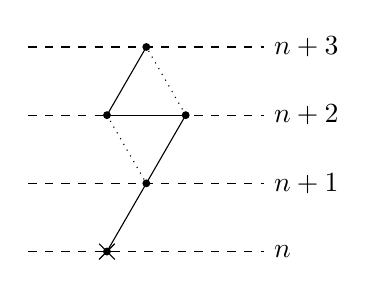
\begin{tikzpicture}
        \begin{scope}[shift=(0 : 0.0)]
          \draw (-0.1,-0.1) -- (0.1,0.1);
          \draw (0.1,-0.1) -- (-0.1,0.1);
          \draw (0 : 0.0) -- (60 : 1.0);
        \end{scope}
      \draw [dashed] (-1.0, 0.0) -- (2.0, 0.0);
      \fill (2.0, 0.0) node [right] {$n$};
      \draw [dashed] (-1.0, 0.866) -- (2.0, 0.866);
      \fill (2.0, 0.866) node [right] {$n+1$};
      \draw [dashed] (-1.0, 1.732) -- (2.0, 1.732);
      \fill (2.0, 1.732) node [right] {$n+2$};
      \draw [dashed] (-1.0, 2.598) -- (2.0, 2.598);
      \fill (2.0, 2.598) node [right] {$n+3$};
      \fill (0,0) circle [radius = 0.05];
      \begin{scope}[shift = (60 : 2.0)]
        \fill(0.0, 0.0) circle [radius = 0.05];
        \foreach \theta in {120, 180, 240}{
          \fill (0.0, 0.0) [transform canvas = {shift = (\theta : 1.0)}] circle [radius = 0.05];
        }
        \draw [dotted] (0 : 0.0) -- (120 : 1.0);
        \draw (0 : 0.0) -- (180 : 1.0);
        \draw (0 : 0.0) -- (240 : 1.0);
      \end{scope}
      \begin{scope}[shift = (60 : 1.0)]
        \begin{scope}[shift = (120 : 1.0)]
          \draw (0.0, 0.0) -- (60 : 1.0);
          \draw [dotted] (0.0, 0.0) -- (300 : 1.0);
        \end{scope}
      \end{scope}
    \end{tikzpicture}

    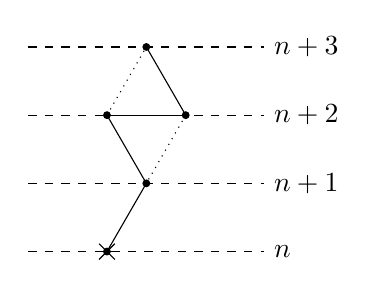
\begin{tikzpicture}
        \begin{scope}[shift=(0 : 0.0)]
          \draw (-0.1,-0.1) -- (0.1,0.1);
          \draw (0.1,-0.1) -- (-0.1,0.1);
          \draw (0 : 0.0) -- (60 : 1.0);
        \end{scope}
      \draw [dashed] (-1.0, 0.0) -- (2.0, 0.0);
      \fill (2.0, 0.0) node [right] {$n$};
      \draw [dashed] (-1.0, 0.866) -- (2.0, 0.866);
      \fill (2.0, 0.866) node [right] {$n+1$};
      \draw [dashed] (-1.0, 1.732) -- (2.0, 1.732);
      \fill (2.0, 1.732) node [right] {$n+2$};
      \draw [dashed] (-1.0, 2.598) -- (2.0, 2.598);
      \fill (2.0, 2.598) node [right] {$n+3$};
      \fill (0,0) circle [radius = 0.05];
      \begin{scope}[shift = (60 : 2.0)]
        \fill(0.0, 0.0) circle [radius = 0.05];
        \foreach \theta in {120, 180, 240}{
          \fill (0.0, 0.0) [transform canvas = {shift = (\theta : 1.0)}] circle [radius = 0.05];
        }
        \draw (0 : 0.0) -- (120 : 1.0);
        \draw (0 : 0.0) -- (180 : 1.0);
        \draw [dotted] (0 : 0.0) -- (240 : 1.0);
      \end{scope}
      \begin{scope}[shift = (60 : 1.0)]
        \begin{scope}[shift = (120 : 1.0)]
          \draw [dotted] (0.0, 0.0) -- (60 : 1.0);
          \draw (0.0, 0.0) -- (300 : 1.0);
        \end{scope}
      \end{scope}
    \end{tikzpicture}
    \end{tabular}
    \caption{}
    \label{fig:afterzigzag}
  \end{center}
\end{figure}

 If they form three bonds once, such as Fig.~\ref{fig:afterline}, the system would need three bonds forever to be deterministic. This becomes nondeterministic finally, such as in Fig.~\ref{fig:hexcorner}, when it reaches a corner of $\hexagon_p^n$. 
 %Therefore, the first fixed bead on a side of an equilateral hexagon with a radius of $n+1$ has to make a hydrogen bond with a molecule on a side of an equilateral hexagon with a radius of $n$.

\begin{figure}
  \begin{center}
  \begin{tabular}{cc}
    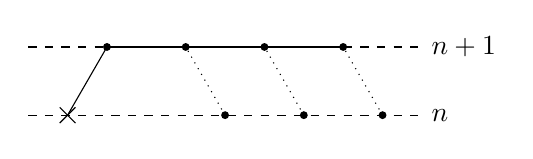
\begin{tikzpicture}
      \begin{scope}[shift=(0 : 0.0)]
        \draw (-0.1,-0.1) -- (0.1,0.1);
        \draw (0.1,-0.1) -- (-0.1,0.1);
        \draw (0 : 0.0) -- (60 : 1.0);
      \end{scope}
      \draw [dashed] (-0.5, 0.0) -- (4.5, 0.0);
      \fill (4.5, 0.0) node [right] {$n$};
      \draw [dashed] (-0.5, 0.866) -- (4.5, 0.866);
      \fill (4.5, 0.866) node [right] {$n+1$};
      \fill (2.0, 0.0) circle [radius = 0.05];
      \fill (3.0, 0.0) circle [radius = 0.05];
      \fill (4.0, 0.0) circle [radius = 0.05];
      \begin{scope}[shift = (60 : 1.0)]
        \fill (0.0, 0.0) circle [radius = 0.05];
        \fill (1.0, 0.0) circle [radius = 0.05];
        \fill (2.0, 0.0) circle [radius = 0.05];
        \fill (3.0, 0.0) circle [radius = 0.05];
        \draw (0.0, 0.0) -- (3.0, 0.0);
      \end{scope}
      \begin{scope}[shift = (0 : 2.0)]
        \draw [dotted] (0 : 0.0) -- (120 : 1.0);
      \end{scope}
      \begin{scope}[shift = (0 : 3.0)]
        \draw [dotted] (0 : 0.0) -- (120 : 1.0);
      \end{scope}
      \begin{scope}[shift = (0 : 4.0)]
        \draw [dotted] (0 : 0.0) -- (120 : 1.0);
      \end{scope}
    \end{tikzpicture}

    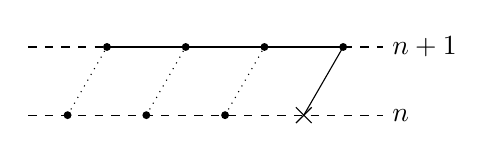
\begin{tikzpicture}
      \begin{scope}[shift=(0 : 0.0)]
        \draw (-0.1,-0.1) -- (0.1,0.1);
        \draw (0.1,-0.1) -- (-0.1,0.1);
        \draw (0 : 0.0) -- (60 : 1.0);
      \end{scope}
      \draw [dashed] (-3.5, 0.0) -- (1.0, 0.0);
      \fill (1.0, 0.0) node [right] {$n$};
      \draw [dashed] (-3.5, 0.866) -- (1.0, 0.866);
      \fill (1.0, 0.866) node [right] {$n+1$};
      \fill (-1.0, 0.0) circle [radius = 0.05];
      \fill (-2.0, 0.0) circle [radius = 0.05];
      \fill (-3.0, 0.0) circle [radius = 0.05];
      \begin{scope}[shift = (60 : 1.0)]
        \fill (0.0, 0.0) circle [radius = 0.05];
        \fill (-1.0, 0.0) circle [radius = 0.05];
        \fill (-2.0, 0.0) circle [radius = 0.05];
        \fill (-3.0, 0.0) circle [radius = 0.05];
        \draw (0.0, 0.0) -- (-3.0, 0.0);
      \end{scope}
      \begin{scope}[shift = (0 : -1.0)]
        \draw [dotted] (0 : 0.0) -- (60 : 1.0);
      \end{scope}
      \begin{scope}[shift = (0 : -2.0)]
        \draw [dotted] (0 : 0.0) -- (60 : 1.0);
      \end{scope}
      \begin{scope}[shift = (0 : -3.0)]
        \draw [dotted] (0 : 0.0) -- (60 : 1.0);
      \end{scope}
    \end{tikzpicture}
    \end{tabular}
    \caption{}
    \label{fig:afterline}
  \end{center}
\end{figure}

Accordingly, it is Fig.~\ref{fig:firstout} when a first bead is fixed on a side of an equilateral hexagon with a radius of $n+1$.

\begin{figure}
  \begin{center}
    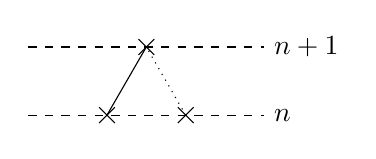
\begin{tikzpicture}
      \draw [dashed] (-1.0, 0.0) -- (2.0, 0.0);
      \fill (2.0, 0.0) node [right] {$n$};
      \draw [dashed] (-1.0, 0.866) -- (2.0, 0.866);
      \fill (2.0, 0.866) node [right] {$n+1$};
      \begin{scope}[shift=(0 : 0.0)]
        \draw (-0.1,-0.1) -- (0.1,0.1);
        \draw (0.1,-0.1) -- (-0.1,0.1);
        \draw (0 : 0.0) -- (60 : 1.0);
      \end{scope}
      \begin{scope}[shift=(60 : 1.0)]
        \draw (-0.1,-0.1) -- (0.1,0.1);
        \draw (0.1,-0.1) -- (-0.1,0.1);
      \end{scope}
      \begin{scope}[shift=(0 : 1.0)]
        \draw (-0.1,-0.1) -- (0.1,0.1);
        \draw (0.1,-0.1) -- (-0.1,0.1);
        \draw [dotted] (0 : 0.0) -- (120 : 1.0);
      \end{scope}
    \end{tikzpicture}
    \caption{}
    \label{fig:firstout}
  \end{center}
\end{figure}

%It has to be a right or left figure in Fig.6. when the first bead fixed on a side of an equilateral hexagon with a radius of $n+1$ make a hydrogen bond with a bead on a side of an equilateral hexagon with a radius of $n$. Fig.6. becomes nondeterministic finally, such as in Fig.7., when it reaches a corner of an equilateral hexagon. It is clear that all beads on a side of an equilateral hexagon with a radius of $n+1$ has to make a hydrogen bond with a bead on a side of an equilateral hexagon with a radius of $n$.  It is impossible to fix molecules on a side of an equilateral hexagon with a radius of $n+2$ and determine the only structure when there are only beads which are able to make a hydrogen bond in an equilateral hexagon with a radius of $n$.



\section{Case of delay $1$}

%%%%%%
\begin{figure}
  \begin{center}
    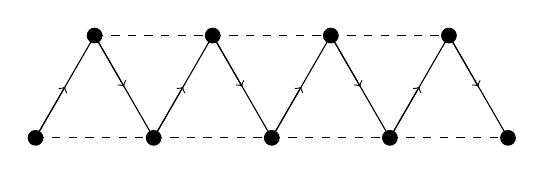
\begin{tikzpicture}
      \fill (0,0) circle[radius = 0.1];
      \fill (1.5,0) circle[radius = 0.1];
      \fill (3,0) circle[radius = 0.1];
      \fill (4.5,0) circle[radius = 0.1];
      \fill (6,0) circle[radius = 0.1];

      \draw[dashed] (0,0)--(1.5,0);
      \draw[dashed] (1.5,0)--(3,0);
      \draw[dashed] (3,0)--(4.5,0);
      \draw[dashed] (4.5,0)--(6,0);
      \draw[->] (0,0)--(60:0.75);
      \draw[->] (1.5,0)--++(60:0.75);
      \draw[->] (3,0)--++(60:0.75);
      \draw[->] (4.5,0)--++(60:0.75);
      \draw (0,0)--(60:1.5);
      \draw (1.5,0)--++(60:1.5);
      \draw (3,0)--++(60:1.5);
      \draw (4.5,0)--++(60:1.5);
      
      \begin{scope}[shift=(60:1.5)]
        \fill (0,0) circle[radius = 0.1];
        \fill (1.5,0) circle[radius = 0.1];
        \fill (3,0) circle[radius = 0.1];
        \fill (4.5,0) circle[radius = 0.1];
        \draw[dashed] (0,0)--(1.5,0);
        \draw[dashed] (1.5,0)--(3,0);
        \draw[dashed] (3,0)--(4.5,0);
        \draw[->] (0,0)--(-60:0.75);
        \draw[->] (1.5,0)--++(-60:0.75);
        \draw[->] (3,0)--++(-60:0.75);
        \draw[->] (4.5,0)--++(-60:0.75);
        
        \draw (0,0)--(-60:1.5);
        \draw (1.5,0)--++(-60:1.5);
        \draw (3,0)--++(-60:1.5);
        \draw (4.5,0)--++(-60:1.5);
      \end{scope}
      
    \end{tikzpicture}
    \caption{zig-zag conformation}
    \label{TTT_zigzag}
  \end{center}
\end{figure}


In this section, we consider Problem~\ref{prob:det_unary_length} at delay 1. Our result, cases of arity 1 and 3 can only yield finite structures of size $O (n)$, and cases of arity 4 and more can only yield finite structures which is size of $O (n^2)$, and a case of arity 2 can yield infinite structures but they are only the zig-zag conformation shown in Fig.~\ref{TTT_zigzag}. 

%In this section, we prove that unary oritatami system can form infinitely at delay 1 and arity 2 deterministically and moreover that the only infinite conformations which its oritatami system can yield is only the zig-zag conformation shown in Fig.\ref{TTT_zigzag}. 


%Let $\Xi$ be a deterministic oritatami system of delay 1 and arity 2. Assume its seed $\sigma$ consists of $n$ beads.
For $i \geq 0$ let $C_i$ be the unique elongation of $\sigma$ by $w[1..i]$, that is, foldable by $\Xi$. Hence $C_0 = \sigma$.


Let us consider the stabilization of the $i$-th bead $a_i$ upon $C_{i-1}$. The bead cannot collaborate with any succeeding bead $w[i+1],w[i+2],\cdots$ at delay 1. There are just two ways to get stabilized at delay 1. One way is to be bound to another bead. The other way is through a $tunnel\ section$. A tunnel section consists of four beads that occupy four neighbors of a point (Fig.\ref{TTT_tunnel_intro}). 
Accordingly, how they are stabilized can be described by a sequence $S$ of $b$'s (bound) and $t$'s (tunnel section); priority is given to $t$, that is, $S[i] = t$ if the $i$-th bead $w_i$ is stabilized not only by being bound but also through a tunnel section. 
We let $S$ take the value $\blacksquare$ for halt.

Assume that four of the six neighbors of a point $p$ are occupied by beads $a_{j_1},a_{j_2},a_{j_3},a_{j_4}$ while the other two are free. We call such a point $p$ the $inside\ of\ a\ tunnel$ and points $p^\prime$ the $entrance\ of\ a\ tunnel$ except when $p^\prime$ is inside of a tunnel. If the beads $w[i-2]$ and $w[i-1]$ are stabilized respectively at one of the two free neighbors and at $p$ one after another, then the next bead $w[i]$ cannot help but be stabilized at the other free neighbor. In this way, $w[i]$ can get stabilized without being bound.

%If a bead is stabilized through a tunnel section, then it can provide some bonds. Let us consider bonds of $C_i$. $C_i$ is represented $C = (W,P,H)$ where $|W| = i + n$ $C_i$ contains $\alpha \cdot (i + n) - 2|H|$ bonds because $C_i$ consists of $i + n$ beads and a bead has just $\alpha$ bonds and then $2 |H|$ of the those bonds are already used. However, even if a bead has an available bond, $w[j]$ $(j > i)$ might not be able to use this bond because the bond has possibility that it is blocked by transcripts $w[i+1..j-1]$. Number of $binding\ capabilities$ does not contain that case so that it is at most $\alpha \cdot (i + n) - 2|H|$.

We say that point $p$ is reachable from a conformation $C$ if there exists a directed path $P^\prime$ from the last point of $C$ that does not cross the path of $C$. We define $binding\ capability$ with reachable.

\begin{definition}[binding capability]
Let $C = (P,w,H)$ be a conformation.
Let $B_k$ be $H \cap \{ (i,j) \mid \mbox{$i=k$ or $j=k$} \}$. Moreover, let $R_k$ be a set of neighbors of the point $P[k]$ that are free and reachable from $C$.
 The binding capability of $C$, denoted by $\#bc(C)$, is defined by $\sum^{|w|}_{k=1} \min \{ |B_k|, |R_k|  \}$.
\end{definition}


\begin{figure}
  \begin{center}
    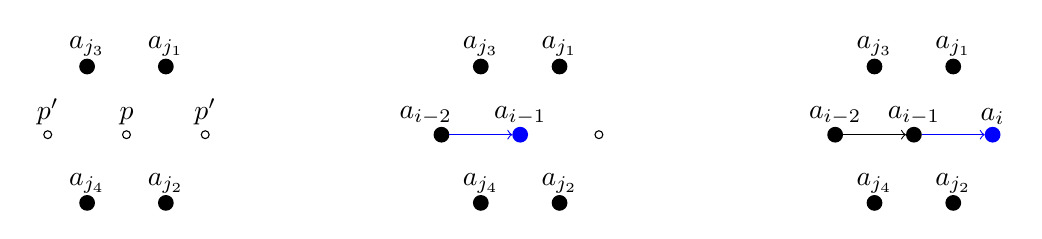
\begin{tikzpicture}
      \draw (0:0) circle [radius=0.05];
      \draw (0:1) circle [radius=0.05];
      \draw (180:1) circle [radius=0.05];
      \node[above] at (0:1) { $p^\prime$ };
      \node[above] at (0:0) { $p$ };
      \node[above] at (180:1) { $p^\prime$ };
      
      \fill (60 : 1) circle [radius=0.1];
      \fill (-60 : 1) circle [radius=0.1];
      \fill (120 : 1) circle [radius=0.1];
      \fill (-120 : 1) circle [radius=0.1];
      \node[above] at (60 :1) { $a_{j_1}$ };
      \node[above] at (-60 :1) { $a_{j_2}$ };
      \node[above] at (120 :1) { $a_{j_3}$ };
      \node[above] at (-120 :1) { $a_{j_4}$ };
      
      \begin{scope}[shift=(0:5)]
        \fill[blue] (0:0) circle [radius=0.1];
        \draw (0:1) circle [radius=0.05];
        \fill (180:1) circle [radius=0.1];
        \node[above] at (180:1.2) { $a_{i-2}$ };
        \node[above] at (0:0) { $a_{i-1}$ };
        \draw[->, blue] (180:0.9) -- (180:0.1);
        
        \fill (60 : 1) circle [radius=0.1];
        \fill (-60 : 1) circle [radius=0.1];
        \fill (120 : 1) circle [radius=0.1];
        \fill (-120 : 1) circle [radius=0.1];
        \node[above] at (60 :1) { $a_{j_1}$ };
        \node[above] at (-60 :1) { $a_{j_2}$ };
        \node[above] at (120 :1) { $a_{j_3}$ };
        \node[above] at (-120 :1) { $a_{j_4}$ };
      \end{scope}
      \begin{scope}[shift=(0:10)]
        \fill (0:0) circle [radius=0.1];
        \fill[blue] (0:1) circle [radius=0.1];
        \fill (180:1) circle [radius=0.1];
        \node[above] at (180:1) { $a_{i-2}$ };
        \node[above] at (0:0) { $a_{i-1}$ };
        \node[above] at (0:1) { $a_i$ };
        \draw[->] (180:0.9) -- (180:0.1);
        \draw[->,blue] (0:0.1) -- (0:0.9);
        
        \fill (60 : 1) circle [radius=0.1];
        \fill (-60 : 1) circle [radius=0.1];
        \fill (120 : 1) circle [radius=0.1];
        \fill (-120 : 1) circle [radius=0.1];
        \node[above] at (60 :1) { $a_{j_1}$ };
        \node[above] at (-60 :1) { $a_{j_2}$ };
        \node[above] at (120 :1) { $a_{j_3}$ };
        \node[above] at (-120 :1) { $a_{j_4}$ };
      \end{scope}
    \end{tikzpicture} 
    \caption{Through a tunnel section}
    \label{TTT_tunnel_intro}
  \end{center}
\end{figure}


%remark 

\begin{theorem}[Tunnel Troll Theorem]
Let $\Xi$ be a deterministic unary oritatami system of delay $\delta = 1$. 
At arity $\alpha \geq 3$, if $S[k] = t$ and $S[k+1] \neq \blacksquare$, then $\#bc(C_{k-1}) > \#bc(C_k)$.
On the other hand, at arity $\alpha = 2$, if there are indices $i,j$ such that $S[i..j+1]$ is either $bbt^{(j-i-1)}b$ or $bt^\ell bt^{j-i-1-\ell}b$ for some $\ell$, then $\#bc(C_{i-1}) > \#bc(C_j)$.
\end{theorem}

%%%%%%%%%%%%%%%%%%%%%%%%%%%%%%%%%%%%%%%%%%%%%%%%%%%%


\proof%{Proof of Tunnel Troll Theorem}
Each bead in the transcript is bound either inside a tunnel or outside. If a bead is stabilized inside a tunnel, 
then it has at most one free neighbor, and hence its successor it to be stabilized there.
Moreover, if a bead is stabilized outside a tunnel, then its position is either an entrance of a tunnel or not.

Tunnel sections have three possible shapes up to symmetry : straight($S$), obtuse($O$) and acute($A$) turn (Fig. \ref{TTT_tunnel}), and we will consider each of those. 

%\begin{lemma}
%\label{TTT_neighbor_lemma}
%For unary transcripts at $\delta = 1$, if a bead has no free hand, then at least $\alpha + 2$ of its neighbors have to be occpied.
%\end{lemma}


\begin{lemma}
\label{TTT_entrance_Tab}
Let $\Xi$ be a deterministic unary oritatami system at delay $\delta = 1$, arity $\alpha =2$. 
Assume $\Xi$ stabilizes the transcript until $w[i-1]$. If $w[i]$ is stabilized at an entrance point of tunnel $A$ or $B$, then $\#bc(C_{i-1}) > \#bc(C_{i})$.
\end{lemma}

\begin{lemma}
\label{TTT_exit}
Let $\Xi$ be a deterministic unary oritatami system of delay $\delta = 1$. 
Let $w[i]$ be a bead which is stabilized at the exit of a tunnel.
At $\delta = 1, \alpha =2$, if we assume $S[h..i+1] = bt^{(i-h)}b \quad (h<i)$, then $\#bc(C_{h-1}) \geq \#bc(C_i)$ and $\#bc(C_{i-2}) \geq \#bc(C_i)$.
%if we assume $\#bc(C_{i-2}) - \#bc(C_{i-1}) = a$, then $\#bc(C_{i}) - \#bc(C_{i-1}) \leq a$.
On the other hand, if we assume $S[k] = t (k \leq i)$ at $\delta =1, \alpha \geq 3$, then $\#bc(C_{k-1}) > \#bc(C_{k})$.
\end{lemma}

\begin{lemma}
\label{TTT_tunnelC_lemma}
Let $\Xi$ be a deterministic unary oritatami system of delay $\delta = 1$, arity $\alpha = 2$. We assume $S[h..i+1] = bt^{(i-h)}b \quad (1<h<i)$. If at least one of $w[h+1..i]$ is stabilized by tunnel $C$, then $\#bc(C_{h-3}) > \#bc(C_{h+1})$ and $\#bc(C_{h-3}) > \#bc(C_i)$.
\end{lemma}


Let us first consider cases of $\delta \geq 3, \alpha = 1$. These cases are clearly true because of Lemma~\ref{TTT_exit}.


Next, we consider the case of $\delta = 2, \alpha = 1$. We assume there is an index $h$ such that $S[h-1..h+1] = bbt$ or $S[h-1..h+1] = tbt$. According to Lemma~\ref{TTT_entrance_Tab}, if $w[h+1]$ is stabilized by tunnel $A$ or $B$, then $\#bc(C_{h-1}) > \#bc(C_{h})$. Also,  According to Lemma~\ref{TTT_tunnelC_lemma}, if $w[h+1]$ is stabilized by tunnel $C$, then $\#bc(C_{h-3}) > \#bc(C_{h+1})$.
On the other hand, if $S[k..l] = bt^{l-k}b$, then $\#bc(C_{k-1}) \geq \#bc(C_{l})$ because of Lemma~\ref{TTT_exit}. Therefore, if there are indices $i$ and $j$ such that $S[i..j+1] = bbt^{(j-i-1)}b$ or $S[i..j+1] = bt^mbt^nb \quad (m + n = j-i-1)$, then $\#bc(C_{i-1}) > \#bc(C_{j})$.

\qed

\begin{figure}
  \begin{center}
    \begin{tabular}{ccc}
      
      \begin{minipage}{0.3\hsize}
        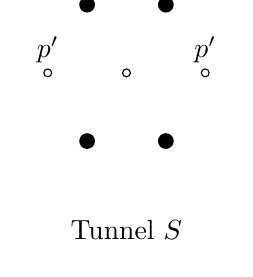
\begin{tikzpicture}
          \begin{scope}[xshift=2cm, yshift=2cm]
            \draw(0,0) circle [radius=0.05];
            \node[above] at (180:1) {$p^\prime$};
            \node[above] at (0:1) {$p^\prime$};

            \foreach \theta in {0,180}{
              \draw[transform canvas={shift=(\theta:1)}](0,0) circle [radius=0.05];
            }
            
            \foreach \theta in {60,-60,120,-120}{
              \fill[transform canvas={shift=(\theta:1)}](0,0) circle [radius=0.1];
            }
          \end{scope}

          \node at (2,0) {Tunnel $S$};
        \end{tikzpicture}
      \end{minipage}

      \begin{minipage}{0.3\hsize}
        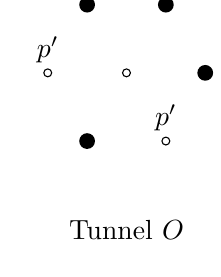
\begin{tikzpicture}

          \begin{scope}[xshift=2cm, yshift=2cm]
            \draw(0,0) circle [radius=0.05];
            \node[above] at (180:1) {$p^\prime$};
            \node[above] at (-60:1) {$p^\prime$};

            \foreach \theta in {-60,180}{
              \draw[transform canvas={shift=(\theta:1)}](0,0) circle [radius=0.05];
            }
            
            \foreach \theta in {0,60,120,-120}{
 	            \fill[transform canvas={shift=(\theta:1)}](0,0) circle [radius=0.1];
            }
          \end{scope}

          \node at (2,0) {Tunnel $O$};
        \end{tikzpicture}
      \end{minipage}

      \begin{minipage}{0.3\hsize}
        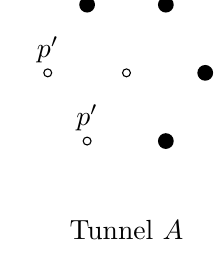
\begin{tikzpicture}

          \begin{scope}[xshift=2cm, yshift=2cm]
            \draw(0,0) circle [radius=0.05];
            \node[above] at (180:1) {$p^\prime$};
            \node[above] at (-120:1) {$p^\prime$};

            \foreach \theta in {-120,180}{
              \draw[transform canvas={shift=(\theta:1)}](0,0) circle [radius=0.05];
            }
            
            \foreach \theta in {0,60,-60,120}{
              \fill[transform canvas={shift=(\theta:1)}](0,0) circle [radius=0.1];
            }
          \end{scope}

          \node at (2,0) {Tunnel $A$};
        \end{tikzpicture}
      \end{minipage}
      
    \end{tabular}
    \caption{All possible tunnel sections: straight, obtuse turn, and acute turn}
    \label{TTT_tunnel}
  \end{center}
\end{figure}



%\begin{figure}
%  \begin{center}
%    \begin{tikzpicture}
%      \draw[thick, gray]
%      (0.5,1)--(0,1)--(0,4)--(4,4)--(4,1)--(3.5,1);
%      \node at(2,1) {Outside};
%      \node at (2,3.2) [rectangle, draw, rounded corners] (enter) {Entrance of a tunnel};
%      \node at(2,1.8) [rectangle, draw, rounded corners] (outside) {Otherwise};
%
%      
%      
%      \draw[thick, gray]
%      (7.5,1)--(7,1)--(7,4)--(11,4)--(11,1)--(10.5,1);
%      \node at(9,1) {Inside of a tunnel};
%      \node at(9,3.2) [rectangle, draw, rounded corners] (next-tunnel) {Successor in inside};
%      \node at(9,1.8) [rectangle, draw, rounded corners] (next-outside) {Successor in outside};
%
%      \draw[->]
%      (outside) edge [bend left, blue] node[left] {$s=b,\Delta=-1$} (enter)
%                   edge [loop left, blue] node[below left] {$s=b,\Delta=\pm 0$} (outside)
%      (enter)   edge [bend left, blue] node[above] {$s=b,\Delta=-1$} (next-tunnel)
%                edge [bend left, blue] node[above] {$s=b,\Delta=-a$} (next-outside)
%                edge [bend left, blue] node[right] {$s=b,\Delta=\pm 0$}  (outside)
%      (next-tunnel) edge[teal]         node[right] {$s=t,\Delta=-a$} (next-outside)
%                edge [loop right, teal]node[right] {$s=t,\Delta=\pm 0$}    (next-tunnel)
%      (next-outside) edge[bend left, teal] node[above] {$s=t,\Delta=+a$}  (outside)
%                edge [bend left, teal]     node[above] {$s=t,\Delta=+(a-1)$}(enter)
%      ;
%      
%    \end{tikzpicture}
%    \caption{Increment on Tunnel A,B}
%    \label{TTT_position}
%  \end{center}
%\end{figure}


%\begin{figure}
%  \begin{center}
%    \begin{tikzpicture}
%      \node at (0,4)   [rectangle, draw,rounded corners] (outside1) {Outside of tunnels};
%      \node at (3.5,4) [rectangle, draw,rounded corners] (enter1)   {Entrance of a tunnel};
%      \node at (7,4)   [rectangle, draw, rounded corners] (inside1) {Inside of a tunnel C};
%      \node at (11,4)  [rectangle, draw, rounded corners] (exit1)   {Inside of a tunnel A or B};
%      \draw[->] (outside1)--(enter1);
%      \draw[->] (enter1)  --(inside1);
%      \draw[->] (inside1) --(exit1);
%      
%      
%      \node at (0,3)   [rectangle, draw,rounded corners] (outside2) {Inside of a tunnel};
%      \node at (3.5,3) [rectangle, draw,rounded corners] (enter2)   {Entrance of a tunnel};
%      \node at (7,3)   [rectangle, draw, rounded corners] (inside2) {Inside of a tunnel C};
%      \node at (11,3)  [rectangle, draw, rounded corners] (exit2)   {Inside of a tunnel A or B};     
%      \draw[->] (outside2)--(enter2);
%      \draw[->] (enter2)  --(inside2);
%      \draw[->] (inside2) --(exit2);
%
%      \node at (0,1)   [rectangle, draw,rounded corners] (outside3) {Outside of tunnels};
%      \node at (3.5,1) [rectangle, draw,rounded corners] (enter3)   {Entrance of a tunnel};
%      \node at (7,1)   [rectangle, draw, rounded corners] (inside3) {Inside of a tunnel C};
%      \node at (11,1)  [rectangle, draw, rounded corners] (exit3)   {Outside of tunnels};     
%      \draw[->] (outside3)--(enter3);
%      \draw[->] (enter3)  --(inside3);
%      \draw[->] (inside3) --(exit3);
%
%      \node at (0,0)   [rectangle, draw,rounded corners] (outside4) {Inside of atunnel};
%      \node at (3.5,0) [rectangle, draw,rounded corners] (enter4)   {Entrance of a tunnel};
%      \node at (7,0)   [rectangle, draw, rounded corners] (inside4) {Inside of a tunnel C};
%      \node at (11,0)  [rectangle, draw, rounded corners] (exit4)   {Outside of tunnels};     
%      \draw[->] (outside4)--(enter4);
%      \draw[->] (enter4)  --(inside4);
%      \draw[->] (inside4) --(exit4);
%    \end{tikzpicture}
%    \caption{Case of Tunnel C}
%    \label{TTT_tunnelC_graph}
%  \end{center}
%\end{figure}


\begin{proof}[lemma \ref{TTT_entrance_Tab}]
Fig.\ref{TTT_tunnel_direction} exhibits all the three kinds of entrance of tunnel A, B.
Let $w[i]$ be stabilized at an entrance point of Tunnel $A$ or $B$.
All cases are $\#bc(C_{i-1}) > \#bc(C_{i})$ as follows.


\begin{itemize}
\item{Case of $t_0$}\\
  Let us consider points $n_3,n_4$. At least one of the points $n_3$ or $n_4$ is free because if both of them are occupied, $p^\prime$ is inside of tunnel. If $n_3$ is free, then $p^\prime$ has to be bound to a bead other than $n_1$ to deterministically stabilize. In this situation, at least three neighbors of $n_1$ are free, that is, $n_1$ has at least one free hand from Lemma~ \ref{TTT_neighbor_lemma}. Hence, $p^\prime$ must be bound to $n_1$. Thus, a case of $t_0$ consumes two hands and it does not supply any binding capabilities.

\item{Case of $t_{\pm 60}$}\\
  In this case, too, $n_4$ or $n_5$ is free. If $n_5$ is free, $p^\prime$ has to be bound to $n_1$ or $n_2$. If $n_5$ is occupied, then $n_4$ is free. This time, by $n_2$ has some free hands so $p^\prime$ has to be bound to $n_2$.
  

  In this situation, $p^\prime$ is able to supply a binding capabilities which could bind a bead into $n_4$ or $n_5$. However, $n_2$ and $n_3$ are part of a contiguous conformation. According to Jordan curve theorem, any successors of $p^\prime$ cannot reach a point $n_4$ or $n_5$ so this capability is inactive. Thus, in the case of $t_{\pm 60}$ $\#bc(C_{i-1}) > \#bc(C_{i})$.

\item{Case of $t_{\pm 120}$}\\
  Binding capabilities that $p^\prime$ supplies are inactive according to Jordan curve theorem on $n_1$ and $n_2$. Moreover, $p^\prime$ has to be bound to one of $n_3, n_4, n_5$ in order to deterministically stabilize.
Thus, in the case of $t_{\pm 120}$ is $\#bc(C_{i-1}) > \#bc(C_{i})$.
  
\end{itemize}

\begin{figure}
  \begin{center}
    \begin{tabular}{ccc}
    
    
      \begin{minipage}{0.3\hsize}
      \centering
        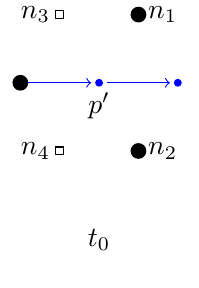
\begin{tikzpicture}
	 \draw[->,white] (120:0.8)--(120:0.1);%for adjustment
          
            \fill[blue] (0,0) circle [radius=0.05];
            \node[below] at (0,0) {$p^\prime$};

            \foreach \theta in {0}{
              \fill[transform canvas={shift=(\theta:1)},blue](0,0) circle [radius=0.05];
            }
            
            \foreach \theta in {60,-60,180}{
              \fill[transform canvas={shift=(\theta:1)}](0,0) circle [radius=0.1];
            }

            \foreach \theta in {120,-120}{
              \draw[transform canvas={shift=(\theta:1)}](-0.05,-0.05) rectangle (0.05,0.05);
            }
            
            \draw[->, blue] (180:0.9)--(180:0.1);
            \draw[->, blue] (0:0.1)--(0:0.9);

            \node[transform canvas={shift=(60:1)},right] {$n_1$};
            \node[transform canvas={shift=(-60:1)},right] {$n_2$};
            \node[transform canvas={shift=(120:1)},left] {$n_3$};
            \node[transform canvas={shift=(-120:1)},left] {$n_4$};


          \node at (0,-2) {$t_{0}$};
        \end{tikzpicture}
      \end{minipage}

      

      \begin{minipage}{0.3\hsize}
      \centering
        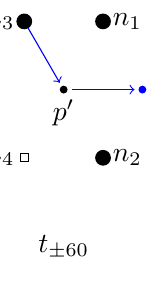
\begin{tikzpicture}

            \fill(0,0) circle [radius=0.05];
            \node[below] at (0,0) {$p^\prime$};

            \foreach \theta in {0}{
              \fill[transform canvas={shift=(\theta:1)},blue](0,0) circle [radius=0.05];
            }
            
            \foreach \theta in {60,-60,120}{
              \fill[transform canvas={shift=(\theta:1)}](0,0) circle [radius=0.1];
            }

            \foreach \theta in {180,-120}{
              \draw[transform canvas={shift=(\theta:1)}](-0.05,-0.05) rectangle (0.05,0.05);
            }
            
            \draw[->, blue] (120:0.9)--(120:0.1);
            \draw[->, blue] (0:0.1)--(0:0.9);

            \node[transform canvas={shift=(60:1)},right] {$n_1$};
            \node[transform canvas={shift=(-60:1)},right] {$n_2$};
            \node[transform canvas={shift=(120:1)},left] {$n_3$};
            \node[transform canvas={shift=(-120:1)},left] {$n_4$};
            \node[transform canvas={shift=(180:1)},left] {$n_5$};

          \node at (0,-2) {$t_{\pm 60}$};
        \end{tikzpicture}
      \end{minipage}

      \begin{minipage}{0.3\hsize}
      \centering
        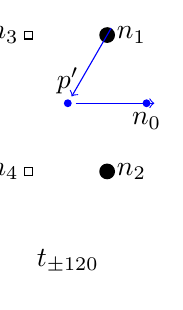
\begin{tikzpicture}
            \fill[blue](0,0) circle [radius=0.05];
            \node[above] at (0,0) {$p^\prime$};

            \foreach \theta in {0}{
              \fill[transform canvas={shift=(\theta:1)}, blue](0,0) circle [radius=0.05];
            }
            
            \foreach \theta in {60,-60}{
              \fill[transform canvas={shift=(\theta:1)}](0,0) circle [radius=0.1];
            }

            \foreach \theta in {180,-120,120}{
              \draw[transform canvas={shift=(\theta:1)}](-0.05,-0.05) rectangle (0.05,0.05);
            }
            
            \draw[->, blue] (60:1.1)--(60:0.1);
            \draw[->, blue] (0:0.1)--(0:1.1);

            \node[transform canvas={shift=(0:1)},below] {$n_0$};
            \node[transform canvas={shift=(60:1)},right] {$n_1$};
            \node[transform canvas={shift=(-60:1)},right] {$n_2$};
            \node[transform canvas={shift=(120:1)},left] {$n_3$};
            \node[transform canvas={shift=(-120:1)},left] {$n_4$};
            \node[transform canvas={shift=(180:1)},left] {$n_5$};

          \node at (0,-2) {$t_{\pm 120}$};
        \end{tikzpicture}
      \end{minipage}
      
    \end{tabular}
    \caption{Direction into a entrance}
    \label{TTT_tunnel_direction}
  \end{center}
\end{figure}

\end{proof}

\begin{proof}[Lemma~ \ref{TTT_exit}]
Fig.\ref{TTT_tunnel_exit} exhibits all the two kinds of exit of tunnel. 
At least one of points $n_1$ or $n_2$ is free because if both of them are occupied, $p^\prime$ is inside of tunnel.

\begin{paragraph}{}
$\delta = 1, \alpha = 2$\\
Let $\Xi$ be a unary oritatami system at $\delta = 1, \alpha = 2$. We assume $S[h..i+1] = bt^{(i-h)}b \quad (h<i)$ and
let $a$ be $\#bc(C_{i-2}) - \#bc(C_{i-1}) = a$. Then, $\#bc(C_{i}) - \#bc(C_{i-1}) \leq a$ as follows. Also, if $i - h > 1$ and $j$ is such that $h<j<i$, then $\#bc(C_{j-1}) \geq \#bc(C_{j})$ because all neighbors of $w[j]$ are occupied by beads forming the tunnel so that any $w[i+1..]$ cannot reach neighbors of $w[j]$. Thus, $\#bc(C_{h-1}) \geq \#bc(C_i)$ and $\#bc(C_{i-2}) \geq \#bc(C_i)$.
\end{paragraph}

\begin{itemize}
\item{Case of both $n_1$ and $n_2$ being free}\\
  This case can be regarded the same as entrance. See Fig.\ref{TTT_tunnel_exit} (Left). Predecessor $n_5$ has to be bound to $n_4$ and $n_5$ because both of $n_3$ and $n_4$ have binding capabilities. Hence, $a \geq 2$. This time, $\alpha = 2$, that is, this case $\#bc(C_{i}) - \#bc(C_{i-1}) \leq a$.
  
\item{Case of $n_1$ is occupied}\\
  See Fig.\ref{TTT_tunnel_exit} (Right). If $n_1$ is occupied, then $n_2$ is free so that $n_5$ has to be bound $n_4$. Hence,  $a \geq 1$. This case can supply two binding capabilities but $p^\prime$ can bind to only one of $n_0$ or $n_2$ because $n_0$ or $n_2$ will be occupied by the successor of $p^\prime$. Therefore, this case $\#bc(C_{i}) - \#bc(C_{i-1}) \leq a$.
  
\end{itemize}

\begin{paragraph}{}
$\delta = 1, \alpha \geq 3$\\
Let $\Xi$ be a unary oritatami system at $\delta = 1, \alpha \geq 3$. We assume $w[i]$ is stabilized at exit of tunnel.
In all cases $\#bc(C_{i-1}) > \#bc(C_{i})$. Moreover, if $S[k] = t (k \leq i)$, then $\#bc(C_{k-1}) > \#bc(C_{k})$ because both sides of the path $p$ in Fig.\ref{TTT_inside_tunnel} ($n_1, n_2$) have two free points and one of $n_1, n_2$ is not the predecessor so that it has hand and moreover that $w[k]$ supplies any binding capabilities because its neighbors are occupied by beads of tunnel.
\end{paragraph}

\begin{itemize}
\item{Case of $n_1$ and $n_2$ are free}\\
  In $\alpha \geq 3$, if three neighbors of a bead leave, then it can supply two binding capabilities. Therefore predecessor $n_5$ has to be bound $n_3$ and $n_4$, and $p^\prime$, too. In this case, at least four bindings are consumed and at most two are added. Thus, it consumes some binding capabilities, overall.
  
\item{Case of $n_1$ is occupied}\\
  In this case, $n_4$ leave at least two bindings and $n_3$, $n_1$ also leave at least one binding. Therefore $n_5$ has to be bound $n_3$ and $n_4$, and $p^\prime$ also has to be bound $n_1$ and $n_4$. In this case, at least four bindings are consumed and at most two are added. Thus, it consumes some binding capabilities, totally.
\end{itemize}


\begin{figure}
  \centering
    \begin{tabular}{cc}
    \begin{minipage}{0.66\hsize}
    \centering
      \begin{tabular}{cc}
      \begin{minipage}{0.45\linewidth}
      \centering
        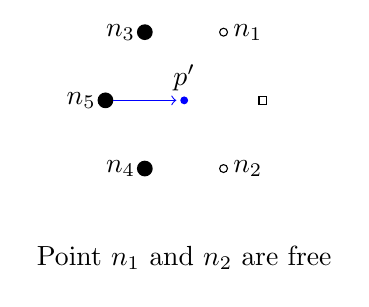
\begin{tikzpicture}
	\draw[white] (0:0) -- (120:1);
	\draw[white] (0:0) -- (-60:1);
	\draw[white] (0:0) -- (0:1);

            \fill[blue](0,0) circle [radius=0.05];
            \node[above] at (0,0) {$p^\prime$};

            
            \foreach \theta in {120,-120,180}{
              \fill[transform canvas={shift=(\theta:1)}](0,0) circle [radius=0.1];
            }

            \foreach \theta in {0}{
              \draw[transform canvas={shift=(\theta:1)}](-0.05,-0.05) rectangle (0.05,0.05);
            }
            \draw (-60:1) circle [radius=0.05];
            \draw (60:1) circle [radius=0.05];

            \draw[->, blue] (180:0.9)--(180:0.1);



            \node[transform canvas={shift=(60:1)},right] {$n_1$};
            \node[transform canvas={shift=(-60:1)},right] {$n_2$};
            \node[transform canvas={shift=(120:1)},left] {$n_3$};
            \node[transform canvas={shift=(-120:1)},left] {$n_4$};
            \node[transform canvas={shift=(180:1)},left] {$n_5$};

          \node at (0,-2) {Point $n_1$ and $n_2$ are free};
        \end{tikzpicture}
      \end{minipage}

      \begin{minipage}{0.45\linewidth}
      \centering
        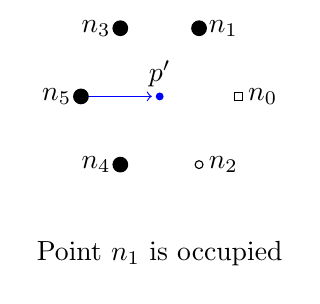
\begin{tikzpicture}
	\draw[white] (0:0) -- (0:1);
	\draw[white] (0:0) -- (120:1);
	\draw[white] (0:0) -- (-90:2);

            \fill[blue](0,0) circle [radius=0.05];
            \node[above] at (0,0) {$p^\prime$};
            
            \foreach \theta in {120,-120,180,60}{
              \fill[transform canvas={shift=(\theta:1)}](0,0) circle [radius=0.1];
            }

            \foreach \theta in {0}{
              \draw[transform canvas={shift=(\theta:1)}](-0.05,-0.05) rectangle (0.05,0.05);
            }
            \draw (-60:1) circle [radius=0.05];

            \draw[->, blue] (180:0.9)--(180:0.1);

            \node[transform canvas={shift=(0:1)},right] {$n_0$};
            \node[transform canvas={shift=(60:1)},right] {$n_1$};
            \node[transform canvas={shift=(-60:1)},right] {$n_2$};
            \node[transform canvas={shift=(120:1)},left] {$n_3$};
            \node[transform canvas={shift=(-120:1)},left] {$n_4$};
            \node[transform canvas={shift=(180:1)},left] {$n_5$};


          
          \node at (0,-2) {Point $n_1$ is occupied};
        \end{tikzpicture}
      \end{minipage}
    \end{tabular}
    \caption{Exit of Tunnel}
    \label{TTT_tunnel_exit}
    \end{minipage}
    
    \begin{minipage}{0.33\hsize}
    \centering
     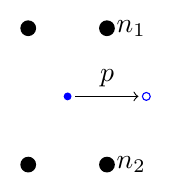
\begin{tikzpicture}
	\draw[white] (0:0) -- (120:1);
	\draw[white] (0:0) -- (-60:1);
            \fill[blue](0,0) circle [radius=0.05];
            \draw[blue] (0:1) circle [radius = 0.05];
            \draw[->] (0:0.1) -- node[above]{$p$} (0:0.9);
            
            \foreach \theta in {60, -60, 120,-120,180}{
              \fill[transform canvas={shift=(\theta:1)}](0,0) circle [radius=0.1];
            }
            \node[transform canvas={shift=(60:1)},right] {$n_1$};
            \node[transform canvas={shift=(-60:1)},right] {$n_2$};
                \end{tikzpicture}
                
    \caption{Inside tunnel}
    \label{TTT_inside_tunnel}
    \end{minipage}
 
    \end{tabular}
\end{figure}
\end{proof}

\begin{proof}[Lemma~ \ref{TTT_tunnelC_lemma}]
Let $\Xi$ be a unary oritatami system at $\delta = 1, \alpha = 2$.
Assume $S[h..i+1] = bt^{i-h}b (h<i)$. If at least one of $w[h+1..i]$ are stabilized by tunnel $C$, then only $w[h+1]$ can use tunnel $C$ because if $w[g]$ which is one of $w[h+2..i]$, with $h+2 \leq g \leq i$ is stabilized by tunnel $C$, $C_g$ is a terminal.


Let us consider stabilization $S[h-1..h+1] = tbt$ or $S[h-1..h+1] = bbt$ as follows. In result, $\#bc(C_{h-3}) > \#bc(C_{h+1})$. In addition according to Lemma~\ref{TTT_exit} $\#bc(C_{h+1}) \geq \#bc(C_{i})$. Thus, $\#bc(C_{h-3}) > \#bc(C_{h+1})$ and $\#bc(C_{h-3}) > \#bc(C_{i})$.
\\

\subsubsection{Case of $S[h-1..h+1] = tbt$}
Fig.\ref{TTT_tunnelC_enter_usingTunnel} exhibits all the two kinds of stabilization depending on structures of tunnel C.

\begin{itemize}
\item{Left of Fig.\ref{TTT_tunnelC_enter_usingTunnel}}\\
  In this figure, Bead $n_4$ has at least one binding so that $w[h-1]$ has to bound $n_4$. Moreover, $w[h]$ has to bind to one of $n_1, n_2, n_3$ in order to stabilize deterministically. On the other hand, $w[h+1]$ can supply two bindings but has only two free neighbors. One of them is occupied by a successor. Therefore $w[h+1]$ can only bind one of $n_5, n_6$, that is, $w[h+1]$ supplies at most one binding. Thus, this case $\#bc(C_{h-1}) > \#bc(C_{h+1})$.

\item{Right of Fig.\ref{TTT_tunnelC_enter_usingTunnel}}\\
  These cases are divided on number of capabilities that $w[h-1]$ consumes.
  \begin{itemize}
  \item[-]{$w[h-1]$ does not consume any bindings}\\
  According to Lemma~\ref{TTT_exit}, $\#bc(C_{h-3}) \geq \#bc(C_{h-1})$ because of $S[h-1] = t$.
    $w[h]$ has to bound one of $n_1, n_2, n_3$ in order to stabilize deterministically so that  $\#bc(C_{h-1}) > \#bc(C_{h})$.
    $w[h+1]$ has to be bound to $w[h-1]$ because $w[h-1]$ has bindings, that is, $w[h+1]$ consumes at least one hand and supplies at most one hand so that $\#bc(C_{h}) \geq \#bc(C_{h+1})$. Thus, in this cases $\#bc(C_{h-3}) > \#bc(C_{h+1})$.
%     This time, let us consider either $n_4$ is occupied or not. If $n_4$ is occupied, then $w[h-1]$ has no active bindings that is this situation consumes some binding capabilities. If $n_4$ is free and $w[h+2]$ is stabilized in $n_4$, then $w[h-1]$ has to bind $w[h+2]$. Therefore, In this case, stabilization of $w[h-1..h+2]$ consumes some bindings. If $n_4$ is free and $w[h+2]$ is stabilized except $n_4$, then this oritatami system has to use two binding capabilities in order to bind $w[h+2]$. Therefore, in this case consumes some bindings. Thus in this cases $\#bc(C_{h-1}) > \#bc(C_{h+2})$.

  \item[-]{$w[h-1]$ consumes one binding}\\
    In this case, $w_{h}$ has to be bound one of $n_1, n_2, n_3$. In addition, $w[h-1]$ and $w[h+1]$ are not supply any bindings. Thus, in this cases consume some binding capabilities.
  \item[-]{$w[h-1]$ consumes two bindings}\\
    In this case, $w[h-1]$ already consumes two binding. $w[h]$ has to be bound. $w[h+1]$ supplies two bindings. Thus, in this cases $\#bc(C_{h-1}) > \#bc(C_{h+1})$.
   
  \end{itemize}
\end{itemize}
\begin{figure}
  \centering
    \begin{tabular}{cc}
      
      \begin{minipage}{0.48\hsize}
      \centering
        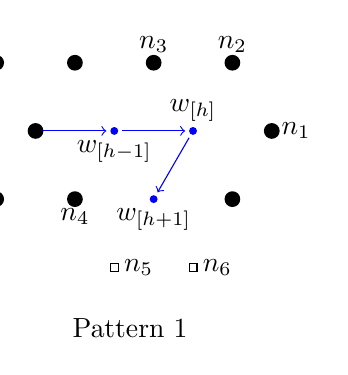
\begin{tikzpicture}

          \fill[transform canvas={shift=(0:0)}](0,0) circle [radius=0.1];
          
          \foreach \theta in {60,-60,120,-120,180}{
            \fill[transform canvas={shift=(\theta:1)}](0,0) circle [radius=0.1];
          }

          \fill[blue](0:1) circle [radius=0.05];
          \draw[->, blue] (0:0.1)--(0:0.9);

          \node[below] at (-60:1) {$n_4$};

          \begin{scope}[shift=(0:2)]
            \fill[blue](0,0) circle [radius=0.05];

            
            \foreach \theta in {120,60,-60,0}{
             \fill[transform canvas={shift=(\theta:1)}](0,0) circle [radius=0.1];
            }

            \draw[->, blue] (180:0.9)--(180:0.1);
            \draw[->, blue] (-120:0.1)--(-120:0.9);

            \node[below] at (180:1) {$w_{[h-1]}$};
            \node[above] at (0:0) {$w_{[h]}$};
            \node[below] at (-120:1) {$w_{[h+1]}$};

            \node[above] at (120:1) {$n_3$};
            \node[above] at (60:1) {$n_2$};
            \node[right] at (0:1) {$n_1$};

            \begin{scope}[shift=(-120:1)]
              \fill[blue](0,0) circle [radius=0.05];
              \foreach \theta in {-120,-60}{
                \draw[transform canvas={shift=(\theta:1)}](-0.05,-0.05) rectangle (0.05,0.05);
              }

              \node[right] at (-120:1) {$n_5$};
              \node[right] at (-60:1) {$n_6$};
            \end{scope}
            
          \end{scope}

          \node at (1.2,-2.5) {Pattern 1};
        \end{tikzpicture}
      \end{minipage}

      \begin{minipage}{0.48\hsize}
      \centering
        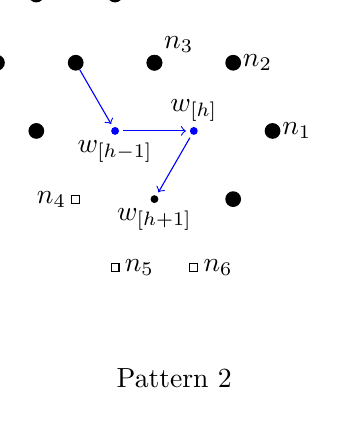
\begin{tikzpicture}

          \fill(0,0) circle [radius=0.1];
          
          \foreach \theta in {60,0,120,-120,180}{
            \fill[transform canvas={shift=(\theta:1)}](0,0) circle [radius=0.1];
          }

          \draw[->, blue] (-60:0.1)--(-60:0.9);


          \begin{scope}[shift=(-60:1),shift=(0:1)]
            \fill[blue](0,0) circle [radius=0.05];
            \fill[blue](180:1) circle [radius=0.05];

            
            \foreach \theta in {120,60,0,-60}{
              \fill[transform canvas={shift=(\theta:1)}](0,0) circle [radius=0.1];
            }

            \draw[->, blue] (180:0.9)--(180:0.1);
            \draw[->, blue] (-120:0.1)--(-120:0.9);

            \node[below] at (180:1) {$w_{[h-1]}$};
            \node[above] at (0:0) {$w_{[h]}$};
            \node[below] at (-120:1) {$w_{[h+1]}$};

            \node[above right] at (120:1) {$n_3$};
            \node[right] at (60:1) {$n_2$};
            \node[right] at (0:1) {$n_1$};

            \begin{scope}[shift=(-120:1)]
              \fill(0,0) circle [radius=0.05];
              \foreach \theta in {180,-120,-60}{
                \draw[transform canvas={shift=(\theta:1)}](-0.05,-0.05) rectangle (0.05,0.05);
              }

              \node[left] at (180:1) {$n_4$};
              \node[right] at (-120:1) {$n_5$};
              \node[right] at (-60:1) {$n_6$};
            \end{scope}
            
          \end{scope}

          \node at (1.25,-4) {Pattern 2};
        \end{tikzpicture}
      \end{minipage}

      
      
    \end{tabular}
    \caption{Case of $S[h-1..h+1] = tbt$}
    \label{TTT_tunnelC_enter_usingTunnel}
\end{figure}


\subsubsection{Case of $S[h-1..h+1] = bbt$}
Let us consider number of consumed bindings by $w[h-1]$ (Fig.\ref{TTT_tunnelC_enter_usingBond}).

\begin{itemize}
\item{$w[h-1]$ consumes one binding}\\
  In this situation, $w[h-1]$ supplies one active binding whereas $w[h+1]$ consumes this binding. In addition, $w[h]$ has to bound to one of $n_1, n_2, n_3$.
  Thus, in this cases consume some binding capabilities.

\item{$w[h-1]$ consumes two bindings}\\
  In this case, $w[h-1]$ already consumes two binding. $w[h]$ has to be bound. $w[h+1]$ supplies at most two bindings. Thus, in this cases consume some binding capabilities.
\end{itemize}



\begin{figure}
  \begin{center}
        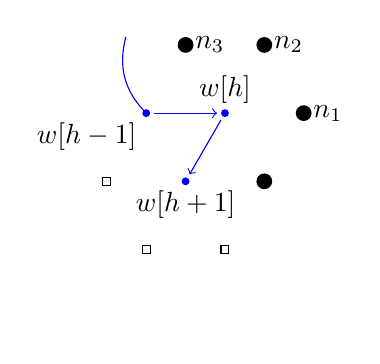
\begin{tikzpicture}
        \draw[->,white] (-70:0.1) -- (-70:3);
          \foreach \theta in {60,-60,120,0}{
            \fill[transform canvas={shift=(\theta:1)}](0,0) circle [radius=0.1];
          }

          \fill[blue](180:1) circle [radius=0.05];
          \fill[blue](0:0) circle [radius=0.05];

          \draw[transform canvas={shift=(180:1)}, blue] (105:1) edge[bend right] (105:0);
          \draw[->, blue] (180:0.9) -- (180:0.1);
          \draw[->, blue] (-120:0.1) -- (-120:0.9);

          \node[below left] at (180:1) {$w[h-1]$};
          \node[above] at (0:0) {$w[h]$};
          \node[below] at (-120:1) {$w[h+1]$};

          \node[right] at (120:1) {$n_3$};
          \node[right] at (60:1) {$n_2$};
          \node[right] at (0:1) {$n_1$};

          \begin{scope}[shift=(-120:1)]
            \fill[blue](0,0) circle [radius=0.05];
            \foreach \theta in {-120,-60,180}{
              \draw[transform canvas={shift=(\theta:1)}](-0.05,-0.05) rectangle (0.05,0.05);
            }
            
          \end{scope}
        \end{tikzpicture}
    \caption{Case of $S[h-1..h+1] = bbt$}
    \label{TTT_tunnelC_enter_usingBond}
  \end{center}
\end{figure}

\end{proof}




%%%%%%%%%%%%%%%%%%%%%%%%%%%%%%%%%%%%%%%%%%%%%%%%%%%%%%%%%
%/////////////////////////////////////////////////
%%%%%%%%%%%%%%%%%%%%%%%%%%%%%%%%%%%%%%%%%%%%%%%%%%%%%%%%%


\subsection{On structures provided by a unary and $\delta = 1$ oritatami system}
\begin{theorem}[$\delta= 1, \alpha=2$]
Let $\Xi$ be a unary oritatami system of $\delta = 1, \alpha = 2$. It can yield infinite structures but they are only zig-zag conformation.
\end{theorem}

\begin{proof}
By Tunnel Troll Theorem, any tunnel sections which represented in $bbt^+$ or $bt^+bt^+$ consume binding capabilities. If the sequence $S$ is free from any subsequence of the form $bt^+bt^+$, then it can factorize as $S = u_1 u_2 u_3 \cdots$ for some $u_1 , u_2 , u_3 , \cdots \in \{b\} \cup bbt^+$. Assume the length of $\sigma$ is $n$, seed supplies at most $2n$ binding capabilities. Therefore formula \ref{TTT_only_bond} hold.

\begin{eqnarray}
  \exists i \in \mathbb{N} \quad s.t. \quad u_{i-1} , u_i , u_{i+1} , u_{i+2} , \cdots \in \{ b \}
  \label{TTT_only_bond}
\end{eqnarray}


Let us represent $S$ as $S[i.i+1...] = v_i v_{i+1} v_{i+2} \cdots$ for some $v_i, v_{i+1}, v_{i+2}, \cdots \in \{ a, o\}$ where if $v_k$ is $a$, then $v_{k+1}$ is bound to $v_{k-1}$, if $v_k$ is $o$, then $v_{k+1}$ is NOT bound to $v_{k-1}$.


Let us consider the case of $v_k$ is $o$. See Fig.\ref{TTT_case_of_o}. $w[i-1]$ consumes some binding capabilities because $v_{i-1}$ is $b$. If the number of $w[i-1]$'s bindings is one binding, then $w[i+1]$ has to be bound except $n_1$ or $n_2$ so that $w[i+1]$ must consumes two bindings except the case of $n_1$ and $n_2$ are occupied and $w[i]$ consumes at least one binding. If $n_1$ and $n_2$ are occupied, then $w[i-1]$'s bindings are inactive, that is, $w[i-1]$ consumes two binding capabilities. Therefore, this case consumes binding capabilities. If $w[i-1]$ dose Not have any bindings, then $w[i-1]$ already consumes two bindings. In addition, $w[i]$ and $w[i+1]$ consume at least one binding. Therefore this case consumes binding capabilities. Thus, the formula \ref{TTT_only_a} hold and according to the formula \ref{TTT_only_bond} and the formula \ref{TTT_only_a}, the formula \ref{TTT_structure} is hold. Thus, in this case, oritatami system can yield infinite structures but they are only zig-zag conformation.

\end{proof}

\begin{eqnarray}
  \exists j \in \mathbb{N} \quad s.t. \quad u_j , u_{j+1} , u_{j+2} , \cdots \in \{ a \}
  \label{TTT_only_a}
\end{eqnarray}

\begin{eqnarray}
  | S | > \forall m \in \mathbb{N} \quad \to \quad \exists n \in \mathbb{N} \quad s.t. \quad S[n], S[n+1], \cdots \in \{ a \}
  \label{TTT_structure}
\end{eqnarray}

\begin{figure}
  \begin{center}
    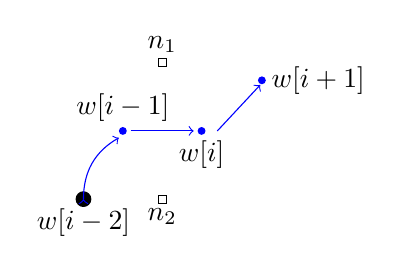
\begin{tikzpicture}
      
      \fill[transform canvas={shift=(-120:1)}](0,0) circle [radius=0.1];
      
      \fill[blue](0:0) circle [radius=0.05];
      \fill[blue](0:1) circle [radius=0.05];
      \fill[shift=(0:1), blue](40:1) circle [radius=0.05];

      \draw[->, blue] (-120:1) edge[bend left] (-120:0.1);
      \draw[->, blue] (0:0.1) -- (0:0.9);
      \draw[->,transform canvas={shift=(0:1.2)}, blue] (50:0) -- (47:0.8);
      
      \draw[shift=(60:1)](-0.05,-0.05) rectangle (0.05,0.05);
      \draw[shift=(-60:1)](-0.05,-0.05) rectangle (0.05,0.05);
      
      \node[below] at (-120:1) {$w[i-2]$};
      \node[above] at (0:0) {$w[i-1]$};
      \node[below] at (0:1) {$w[i]$};
      \node[right, shift=(0:1)] at (40:1) {$w[i+1]$};

      \node[above] at (60:1) {$n_1$};
      \node[below] at (-60:1) {$n_2$};
        
    \end{tikzpicture}
    \caption{Case of $S[i]$}
    \label{TTT_case_of_o}
  \end{center}
\end{figure}

\begin{theorem}[$\delta = 1, \alpha = 3$]
Let $\Xi$ be a unary oritatami system of $\delta = 1, \alpha = 3$. It can yield only finite structures whose size is $\mathcal{O}(n)$.
\end{theorem}

\begin{lemma}
\label{TTT_a3_2b_lemma}
 Let $p$ be a point whose neighbors is occupied at least two point. If $w[i]$ is not stabilized and $w[i-1]$ includes neighbors of $p$, then $w[i]$ is stabilized at $p$ with at least one bond, $w[i]$ is stabilized at another point of $p$ otherwise with at least two bond except any neighbors of $p$ is occupied.
\end{lemma}

\begin{proof}[proof of lemma]
Assume the transcript is stabilized until $w[i-1]$. One of neighbors of $p$ is not $w[i-1]$ where this bead regards $n_1$. If $w[i-1]$ include neighbors of $p$ and $w[i]$ is stabilized at another point of $p$ with one bond. Then, any neighbors do not have bond without $w[i-1]$. Neighbors of $n_1$ have to be occupied at least five according to lemma \ref{TTT_neighbor_lemma} and two of them include neighbors of $p$ where each of them regards $n_2, n_3$. In the same way, five neighbors of $n_2$ and $n_3$ are occupied and each of one of them includes neighbors of $p$ where they regard $n_4, n_5$. one of $n_5$'s neighbors includes neighbors of $p$ where it regards $n_6$. Then, any neighbors of $p$ are occupied. That is, if some neighbors of $p$ are free, then there exists a bead which has bonds in neighbors.
\end{proof}

\begin{proof}
Let us show that $\#bc(C_{i-1}) > \#bc(C_i)$, that is, when $w[i]$ is stabilized, $w[i]$ uses at least two hands.
Let us assume $w[i]$ is able to be stabilized with using one hand. Fig.\ref{TTT_a3_w} exhibits all the three kinds of possibility of stabilized $w[i]$. Then, $w[i]$ can be also stabilized at $n_3$. 

\begin{paragraph}{Case of straight}
\begin{itemize}
\item[-] Case of $n_3$ is free\\
According to assumption, $w[i]$ uses only one hand. Therefore, any neighbors of $n_3$ are occupied according to the lemma\ref{TTT_a3_2b_lemma}. $n_3$ and the point which is stabilized $w[i]$ are free so that $n_1$ has some bond by lemma\ref{TTT_neighbor_lemma}. Accordingly, this situation is non-deterministic. Thus, $n_3$ and $n_4$ have to be occupied because of symmetry.

\item[-] Otherwise\\
Because of  $S[i] = b$, at least one of $n_1$ and $n_2$ have to be free. Let us regard that $n_1$ is free. Neighbors of $n_1$ have to be occupied and at least two neighbors of $n_{-1}$ have to be free for $n_1$ and $w[i]$. According to lemma\ref{TTT_neighbor_lemma}, $n_{-1}$ have some hand. Therefore $w[i]$ can be also stabilized $n_1$, that is, this situation is non-deterministic. Thus, one of $n_3$ and $n_4$ has to be free.
\end{itemize}

Therefore, this case is false.
\end{paragraph}

\begin{paragraph}{Case of obtuse}
\begin{itemize}
\item[-] Case of $n_3$ is free\\
Any neighbors of $n_3$ have to be occupied but the point which is stabilized $w[i]$ is free. Thus $n_3$ has to be occupied.
\item[-] Case of $n_4$ is free\\
According to lemma\ref{TTT_a3_2b_lemma}, $n_2$ has to be occupied because $n_4$ is free. Also $n_0$ has to be occupied from lemma\ref{TTT_neighbor_lemma}. Thus, only one of $n_0, n_3$ leave some hands or both of them do not leave any hands because $w[i]$ use only one bond.\\
If $n_0$ has some hands, then $n_3$ does not have any hands so that $n_{-3}$ is occupied. Also $n_{-3}$ must not have any hands so that $n_{-2}$ is occupied and also $n_{-1}$ is occupied. Therefore any neighbors of $w[i]$ are occupied so that $w[i+1]$ cannot provide.\\
If $n_3$ has some hands, then $n_0$ does not have any hands so that $n_{-1}$ is occupied. In the same previous way, any $n_{-2}, n_{-3}$ are occupied.  Therefore any neighbors of $w[i]$ are occupied.\\
If both of $n_0, n_3$ do not have any hands, then both of $n_{-1}, n_{-3}$ are occupied. If one of $n_{-1}, n_{-3}$ has some hands, the other does not have any hands so that $n_{-2}$ is occupied. If both of $n_{-1}, n_{-3}$ do not have any hands, $n_{-2}$ has to be occupied and $n_{-2}$ has some hands.Therefore any neighbors of $w[i]$ are occupied so that $w[i+1]$ cannot provide.\\
Thus $n_3$ has to be occupied in order to yield infinite structures.
\item[-] Case of $n_2$ is free\\
Any neighbors of $n_2$ have to be occupied so that $n_0$ is occupied. Any neighbors of $n_0$ except $n_2$ have to be also occupied but the point which is stabilized $w[i]$ is free. Thus $n_2$ has to be occupied.
\item[-] Case of $n_0$ is free\\
Any neighbors of $n_0$ have to be occupied so that $n_{-1}$ is occupied. Any neighbors of $n_{-1}$ except $n_0$ have to be also occupied but the point which is stabilized $w[i]$ is free. Thus $n_0$ has to be occupied. 
\end{itemize}

Therefore, any situations contradict $S[i] = b$.

\end{paragraph}



\begin{paragraph}{Case of acute}
\begin{itemize}
\item[-] Case of $n_4$ is free\\
$n_4$ and a point which is stabilized $w[i]$ are free so that  $w[i-2]$ has some hands according to lemma\ref{TTT_neighbor_lemma}.
However, $w[i]$ can be also stabilized $n_4$ in this case. Thus, $n_4$ has to be occupied.
\item[-] Case of $n_2$ is free\\
According to lemma\ref{TTT_a3_2b_lemma}, $n_0$ has to be occupied. $n_1$ has to be also occupied because of lemma\ref{TTT_neighbor_lemma}.
We consider this case just like case of obtuse and that $n_4$ is free. Then if $w[i-2]$ binds $w[i]$, any $n_{-1}, n_{-2}, n_{-3}$ are occupied. If $n_1$ binds $w[i]$, this case is same. Also if $n_1$ and $w[i-2]$ do not have any hand, any $n_{-1}, n_{-2}, n_{-3}$ are occupied. Therefore, $w[i+1]$ cannot be provided.
\item[-] Case of $n_0$ is free\\
Any neighbors of $n_0$ have to be occupied so that $n_{1}$ is occupied. Any neighbors of $n_{1}$ except $n_0$ have to be also occupied but the point which is stabilized $w[i]$ is free. Thus $n_0$ has to be occupied. 
\item[-] Case of $n_1$ is free\\
Any neighbors of $n_1$ have to be occupied so that $n_{-1}$ is occupied. Any neighbors of $n_{-1}$ except $n_1$ have to be also occupied but the point which is stabilized $w[i]$ is free. Thus $n_1$ has to be occupied. 
\end{itemize}

Therefore, any situations contradict $S[i] = b$.
\end{paragraph}\\


Hence, assumption that w[i] is able to be stabilized with using one hand is false.
Therefore, when w[i] is stabilized, w[i] uses at least two hands.
\end{proof}

\begin{figure}
  \begin{center}
  \begin{tabular}{c c c}
 \begin{minipage}{0.3\hsize}
 \centering
    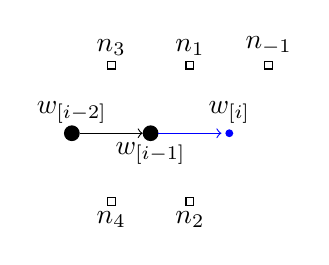
\begin{tikzpicture}
      
      \fill[shift=(180:1)] (0,0) circle [radius=0.1];
      \fill[shift=(180:0)] (0,0) circle [radius=0.1];
      
      \fill[blue](0:1) circle [radius=0.05];
      
      \draw[->] (180:0.9) -- (180:0.1);
      \draw[->, blue] (0:0.1) -- (0:0.9);

	\node[above] at (180:1) {$w_{[i-2]}$};
	\node[below] at (180:0) {$w_{[i-1]}$};
	\node[above] at (0:1) {$w_{[i]}$};

	\foreach \theta in {60,-60,120,-120}{
   	   \draw [shift=(\theta:1)] (-0.05,-0.05) rectangle (0.05,0.05);
  	}
	 \draw [shift=(60:1)] (0.95,-0.05) rectangle (1.05,0.05);
 	\node[above] at (60:1) {$n_1$};
	\node[below] at (-60:1) {$n_2$};
	\node[above] at (120:1) {$n_3$};
	\node[below] at (-120:1) {$n_4$};
	\node[above, shift=(0:1)] at (60:1) {$n_{-1}$};
    \end{tikzpicture}
    \end{minipage}
    
    \begin{minipage}{0.3\hsize}
    \centering
     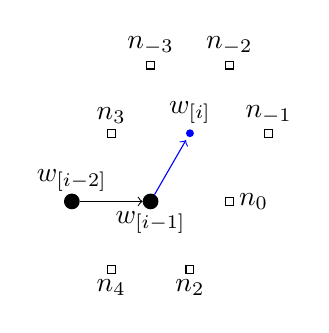
\begin{tikzpicture}
      
      \fill[shift=(180:1)] (0,0) circle [radius=0.1];
      \fill[shift=(180:0)] (0,0) circle [radius=0.1];
      
      \fill[blue](60:1) circle [radius=0.05];
      
      \draw[->] (180:0.9) -- (180:0.1);
      \draw[->, blue] (60:0.1) -- (60:0.9);

	\node[above] at (180:1) {$w_{[i-2]}$};
	\node[below] at (180:0) {$w_{[i-1]}$};
	\node[above] at (60:1) {$w_{[i]}$};


	\foreach \theta in {0,-60,120,-120}{
   	   \draw [shift=(\theta:1)] (-0.05,-0.05) rectangle (0.05,0.05);
  	}
	\draw [shift=(60:1)] (0.95,-0.05) rectangle (1.05,0.05);
	\draw [shift=(60:1), shift=(60:1)] (-0.05,-0.05) rectangle (0.05,0.05);
	\draw [shift=(60:1), shift=(120:1)] (-0.05,-0.05) rectangle (0.05,0.05);
	
 	\node[right] at (0:1) {$n_0$};
	\node[below] at (-60:1) {$n_2$};
	\node[above] at (120:1) {$n_3$};
	\node[below] at (-120:1) {$n_4$};
	\node[above, shift=(0:1)] at (60:1) {$n_{-1}$};
	\node[above, shift=(60:1)] at (60:1) {$n_{-2}$};
	\node[above, shift=(60:1)] at (120:1) {$n_{-3}$};
    \end{tikzpicture}
    \end{minipage}
    
    \begin{minipage}{0.3\hsize}
        \centering
     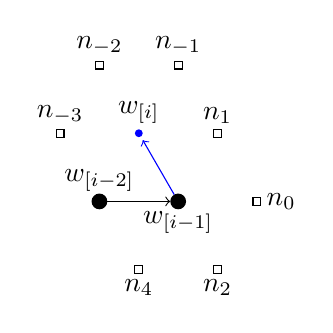
\begin{tikzpicture}
      
      \fill[shift=(180:1)] (0,0) circle [radius=0.1];
      \fill[shift=(180:0)] (0,0) circle [radius=0.1];
      
      \fill[blue](120:1) circle [radius=0.05];
      
      \draw[->] (180:0.9) -- (180:0.1);
      \draw[->, blue] (120:0.1) -- (120:0.9);

	\node[above] at (180:1) {$w_{[i-2]}$};
	\node[below] at (180:0) {$w_{[i-1]}$};
	\node[above] at (120:1) {$w_{[i]}$};


	\foreach \theta in {0,60,-60,-120}{
   	   \draw [shift=(\theta:1)] (-0.05,-0.05) rectangle (0.05,0.05);
  	}
	\draw [shift=(120:1), shift=(60:1)] (-0.05,-0.05) rectangle (0.05,0.05);
	\draw [shift=(120:1), shift=(120:1)] (-0.05,-0.05) rectangle (0.05,0.05);
	\draw [shift=(120:1), shift=(180:1)] (-0.05,-0.05) rectangle (0.05,0.05);
	
 	\node[right] at (0:1) {$n_0$};
	\node[above] at (60:1) {$n_1$};
	\node[below] at (-60:1) {$n_2$};
	\node[below] at (-120:1) {$n_4$};
	\node[above, shift=(120:1)] at (60:1) {$n_{-1}$};
	\node[above, shift=(120:1)] at (120:1) {$n_{-2}$};
	\node[above, shift=(120:1)] at (180:1) {$n_{-3}$};
    \end{tikzpicture}
    \end{minipage}
    \end{tabular}
    \caption{All possible directions of $w[i]$: straight, obtuse, acute.}
    \label{TTT_a3_w}
  \end{center}
\end{figure}

\begin{theorem}[$\delta = 1, \alpha = 4$]
Let $\Xi$ be a unary oritatami system of $\delta = 1, \alpha = 4$. It can yield only finite structures whose size is $\mathcal{O}(n^2)$.
\end{theorem}

\begin{lemma}
\label{TTT_a4_2b_lemma}
Any beads which are already stabilized by some bonds use at least two bonds.
\end{lemma}

\begin{proof}[proof of lemma]
Let us consider when $w[i]$ is stabilized by only one bond. See Fig.\ref{TTT_a4_lemma_fig}. According to lemma\ref{TTT_neighbor_lemma}, if $n_3$ is free, $w[i-2]$ has some hands. Thus, $n_4$ has to be occupied in order to stabilize deterministically. Moreover, also $n_2$ has to be occupied for deterministic and also $n_0, n_1$. $n_1$ has some hands because $n_3$ is free. Therefore, $w[i]$ is stabilized at $n_3$ and it has to use at least two hands. It contradict assumption.
\end{proof}

\begin{proof}
According to lemma\ref{TTT_a4_2b_lemma}, when $w[i]$ is stabilized, it has to use at least two bonds. Let us consider when a bead $w[i]$ which is the first bead out of $\hexagon_{w[-n+1]}^n$ is stabilized. See Fig.\ref{TTT_a4_first}. any $n_0, n_1, n_3, n_5$ is free because if some of them is occupied, $w[i]$ is not the first bead out of $\hexagon_{w[-n+1]}^n$. At least two neighbors of $w[i]$ except predecessor have to be occupied in order to bind. In this case, a point which is able to put a bead is only $n_2$. Therefore, any transcript cannot be stabilized in out of $\hexagon_{w[-n+1]}^n$. Hence oritatami system can yield only a finite structure whose size is $\mathcal{O}(n^2)$ in $\delta =1, \alpha = 4$.
%lemma???a=4??#bc(C_i) >= #bc(C_{i+1})? ?upper?left
\end{proof}


\begin{figure}
 \centering
    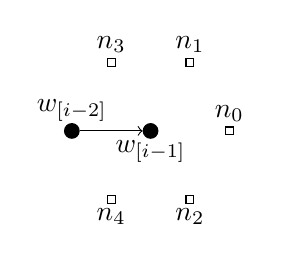
\begin{tikzpicture}
	\fill[shift=(180:1)] (0,0) circle [radius=0.1];
      \fill[shift=(180:0)] (0,0) circle [radius=0.1];
      
      \draw[->] (180:0.9) -- (180:0.1);

	\node[above] at (180:1) {$w_{[i-2]}$};
	\node[below] at (180:0) {$w_{[i-1]}$};
	\node[above] at (0:1) {$n_0$};

	\foreach \theta in {0,60,-60,120,-120}{
   	   \draw [shift=(\theta:1)] (-0.05,-0.05) rectangle (0.05,0.05);
  	}
 	\node[above] at (60:1) {$n_1$};
	\node[below] at (-60:1) {$n_2$};
	\node[above] at (120:1) {$n_3$};
	\node[below] at (-120:1) {$n_4$};
    \end{tikzpicture}
    \caption{$\alpha = 4$: when $w[i]$ is stabilized}
    \label{TTT_a4_lemma_fig}
\end{figure}

\begin{figure}
 \centering
    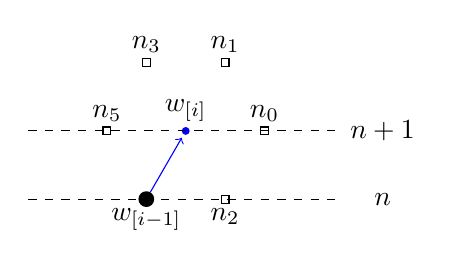
\begin{tikzpicture}
	\fill[shift=(-120:1)] (0,0) circle [radius=0.1];
      \fill[shift=(180:0), blue] (0,0) circle [radius=0.05];
      
      \draw[dashed] (180:2) -- (0:2);
      \draw[dashed, shift=(-60:1)] (180:2.5) -- (0:1.5);
      \draw[->, blue] (-120:0.9) -- (-120:0.1);

	\node[below] at (-120:1) {$w_{[i-1]}$};
	\node[above] at (180:0) {$w_{[i]}$};
	\node[above] at (0:1) {$n_0$};

	\foreach \theta in {0,60,-60,120,180}{
   	   \draw [shift=(\theta:1)] (-0.05,-0.05) rectangle (0.05,0.05);
  	}

 	\node[above] at (60:1) {$n_1$};
	\node[below] at (-60:1) {$n_2$};
	\node[above] at (120:1) {$n_3$};
	\node[above] at (180:1) {$n_5$};
	
	\node at (0:2.5) {$n+1$};
	\node[shift=(-60:1)] at (0:2) {$n$};
    \end{tikzpicture}
    \caption{the first bead out of $\hexagon_{w[-n+1]}^n$}
    \label{TTT_a4_first}
\end{figure}






\bibliographystyle{splncs03}
\bibliography{tamc2019.bib}
  
\end{document}
